%%
%% This is file `sample-sigplan.tex',
%% generated with the docstrip utility.
%%
%% The original source files were:
%%
%% samples.dtx  (with options: `all,proceedings,bibtex,sigplan')
%% 
%% IMPORTANT NOTICE:
%% 
%% For the copyright see the source file.
%% 
%% Any modified versions of this file must be renamed
%% with new filenames distinct from sample-sigplan.tex.
%% 
%% For distribution of the original source see the terms
%% for copying and modification in the file samples.dtx.
%% 
%% This generated file may be distributed as long as the
%% original source files, as listed above, are part of the
%% same distribution. (The sources need not necessarily be
%% in the same archive or directory.)
%%
%%
%% Commands for TeXCount
%TC:macro \cite [option:text,text]
%TC:macro \citep [option:text,text]
%TC:macro \citet [option:text,text]
%TC:envir table 0 1
%TC:envir table* 0 1
%TC:envir tabular [ignore] word
%TC:envir displaymath 0 word
%TC:envir math 0 word
%TC:envir comment 0 0
%%
%%
%% The first command in your LaTeX source must be the \documentclass
%% command.
%%
%% For submission and review of your manuscript please change the
%% command to \documentclass[manuscript, screen, review]{acmart}.
%%
%% When submitting camera ready or to TAPS, please change the command
%% to \documentclass[sigconf]{acmart} or whichever template is required
%% for your publication.
%%
%%
\documentclass[sigplan,twocolumn,review,anonymous]{acmart}
\acmSubmissionID{841}
\renewcommand\footnotetextcopyrightpermission[1]{}
\usepackage[]{hyperref}
\usepackage{xcolor}
\newcommand{\MYhref}[3][blue]{\href{#2}{\color{#1}{#3}}}%
\usepackage{graphicx}
\usepackage{rotating}
\usepackage{float}
\DeclareGraphicsExtensions{.pdf,.png,.jpg}
\usepackage{subfig}
\usepackage[ruled,linesnumbered]{algorithm2e}
\usepackage{booktabs}
\usepackage{multirow}
\usepackage[ruled,linesnumbered]{algorithm2e}
\newcommand{\myparagraph}[1]{\textbf{#1.}}
\setlength{\parskip}{0pt}
% Optional: Remove the ACM reference between the abstract and the main text.
\settopmatter{printfolios=true,printacmref=false}
% Optional: Comment out the CCS concepts and keywords.

%%
%% \BibTeX command to typeset BibTeX logo in the docs
\AtBeginDocument{%
  \providecommand\BibTeX{{%
    Bib\TeX}}}

%% Rights management information.  This information is sent to you
%% when you complete the rights form.  These commands have SAMPLE
%% values in them; it is your responsibility as an author to replace
%% the commands and values with those provided to you when you
%% complete the rights form.
\setcopyright{acmlicensed}
\copyrightyear{2018}
\acmYear{2018}
\acmDOI{XXXXXXX.XXXXXXX}

%% These commands are for a PROCEEDINGS abstract or paper.
\acmConference[EuroSys '25]{EuroSys}{March 30--April 3, 2025}{ROTTERDAM}
%%
%%  Uncomment \acmBooktitle if the title of the proceedings is different
%%  from ``Proceedings of ...''!
%%
%%\acmBooktitle{Woodstock '18: ACM Symposium on Neural Gaze Detection,
%%  June 03--05, 2018, Woodstock, NY}
\acmISBN{978-1-4503-XXXX-X/18/06}


%%
%% Submission ID.
%% Use this when submitting an article to a sponsored event. You'll
%% receive a unique submission ID from the organizers
%% of the event, and this ID should be used as the parameter to this command.
%%\acmSubmissionID{123-A56-BU3}

%%
%% For managing citations, it is recommended to use bibliography
%% files in BibTeX format.
%%
%% You can then either use BibTeX with the ACM-Reference-Format style,
%% or BibLaTeX with the acmnumeric or acmauthoryear sytles, that include
%% support for advanced citation of software artefact from the
%% biblatex-software package, also separately available on CTAN.
%%
%% Look at the sample-*-biblatex.tex files for templates showcasing
%% the biblatex styles.
%%

%%
%% The majority of ACM publications use numbered citations and
%% references.  The command \citestyle{authoryear} switches to the
%% "author year" style.
%%
%% If you are preparing content for an event
%% sponsored by ACM SIGGRAPH, you must use the "author year" style of
%% citations and references.
%% Uncommenting
%% the next command will enable that style.
%%\citestyle{acmauthoryear}


%%
%% end of the preamble, start of the body of the document source.
\begin{document}

%%
%% The "title" command has an optional parameter,
%% allowing the author to define a "short title" to be used in page headers.
\title{CacheInf: Collaborative Edge-Cloud Cache System for Efficient Robotic Visual Model Inference}

%%
%% The "author" command and its associated commands are used to define
%% the authors and their affiliations.
%% Of note is the shared affiliation of the first two authors, and the
%% "authornote" and "authornotemark" commands
%% used to denote shared contribution to the research.
% \author{Ben Trovato}
% \authornote{Both authors contributed equally to this research.}
% \email{trovato@corporation.com}
% \orcid{1234-5678-9012}
% \author{G.K.M. Tobin}
% \authornotemark[1]
% \email{webmaster@marysville-ohio.com}
% \affiliation{%
%   \institution{Institute for Clarity in Documentation}
%   \city{Dublin}
%   \state{Ohio}
%   \country{USA}
% }

% \author{Lars Th{\o}rv{\"a}ld}
% \affiliation{%
%   \institution{The Th{\o}rv{\"a}ld Group}
%   \city{Hekla}
%   \country{Iceland}}
% \email{larst@affiliation.org}

% \author{Valerie B\'eranger}
% \affiliation{%
%   \institution{Inria Paris-Rocquencourt}
%   \city{Rocquencourt}
%   \country{France}
% }

% \author{Aparna Patel}
% \affiliation{%
%  \institution{Rajiv Gandhi University}
%  \city{Doimukh}
%  \state{Arunachal Pradesh}
%  \country{India}}

% \author{Huifen Chan}
% \affiliation{%
%   \institution{Tsinghua University}
%   \city{Haidian Qu}
%   \state{Beijing Shi}
%   \country{China}}

% \author{Charles Palmer}
% \affiliation{%
%   \institution{Palmer Research Laboratories}
%   \city{San Antonio}
%   \state{Texas}
%   \country{USA}}
% \email{cpalmer@prl.com}

% \author{John Smith}
% \affiliation{%
%   \institution{The Th{\o}rv{\"a}ld Group}
%   \city{Hekla}
%   \country{Iceland}}
% \email{jsmith@affiliation.org}

% \author{Julius P. Kumquat}
% \affiliation{%
%   \institution{The Kumquat Consortium}
%   \city{New York}
%   \country{USA}}
% \email{jpkumquat@consortium.net}

%%
%% By default, the full list of authors will be used in the page
%% headers. Often, this list is too long, and will overlap
%% other information printed in the page headers. This command allows
%% the author to define a more concise list
%% of authors' names for this purpose.
% \renewcommand{\shortauthors}{Trovato et al.}

%%
%% The abstract is a short summary of the work to be presented in the
%% article.

\begin{abstract}
Visual information processing is crucial for mobile robots performing tasks such as navigation, manipulation, and human-robot interaction. However, limited computational power for local computation and unstable wireless network bandwidth for computation offloading to a GPU server on these robots lead to slow visual model inference, hindering real-time responsiveness and increasing energy consumption. Existing caching mechanisms designed for fixed edge devices reduce computation by reusing cached activations (computation intermediates) by aligning the activations to the detected movements on the input images, but they face challenges on mobile robots due to frequent camera perspective changes that accumulates error when reusing the cached activation, which leads to degraded inference accuracy or frequent discarding and recomputing the cached activations that increases latency.

We propose CacheInf, a high-performance edge-cloud caching system for efficient visual model inference on mobile robots. Instead of wholly reusing or recomputing the activations, CacheInf selectively reuses a portion of the cached activations frame and recomputes the others, which minimizes required computation, accelerates both local processing and computation offloading, and mitigates error accumulation in activations, achieving an optimal trade-off between inference accuracy and speed.
Evaluation on various visual models and wireless network environments shows CacheInf reduced end-to-end inference latency by up to 48.8\% and reduced average energy consumption for inference by up to 39.9\% compared with the baselines.

\end{abstract}

%%
%% The code below is generated by the tool at http://dl.acm.org/ccs.cfm.
%% Please copy and paste the code instead of the example below.
%%
% \begin{CCSXML}
% <ccs2012>
%  <concept>
%   <concept_id>00000000.0000000.0000000</concept_id>
%   <concept_desc>Do Not Use This Code, Generate the Correct Terms for Your Paper</concept_desc>
%   <concept_significance>500</concept_significance>
%  </concept>
%  <concept>
%   <concept_id>00000000.00000000.00000000</concept_id>
%   <concept_desc>Do Not Use This Code, Generate the Correct Terms for Your Paper</concept_desc>
%   <concept_significance>300</concept_significance>
%  </concept>
%  <concept>
%   <concept_id>00000000.00000000.00000000</concept_id>
%   <concept_desc>Do Not Use This Code, Generate the Correct Terms for Your Paper</concept_desc>
%   <concept_significance>100</concept_significance>
%  </concept>
%  <concept>
%   <concept_id>00000000.00000000.00000000</concept_id>
%   <concept_desc>Do Not Use This Code, Generate the Correct Terms for Your Paper</concept_desc>
%   <concept_significance>100</concept_significance>
%  </concept>
% </ccs2012>
% \end{CCSXML}

% \ccsdesc[500]{Do Not Use This Code~Generate the Correct Terms for Your Paper}
% \ccsdesc[300]{Do Not Use This Code~Generate the Correct Terms for Your Paper}
% \ccsdesc{Do Not Use This Code~Generate the Correct Terms for Your Paper}
% \ccsdesc[100]{Do Not Use This Code~Generate the Correct Terms for Your Paper}

%%
%% Keywords. The author(s) should pick words that accurately describe
%% the work being presented. Separate the keywords with commas.
\keywords{Edge computing}
%% A "teaser" image appears between the author and affiliation
%% information and the body of the document, and typically spans the
%% page.

%%
%% This command processes the author and affiliation and title
%% information and builds the first part of the formatted document.
\maketitle



\section{Introduction}
Visual information is vital for various robotic tasks deployed on real-world edge devices (typically mobile robots), such as navigation~\cite{ran2017convolutional}, manipulation~\cite{bayar2018constrained}, and human-robot interaction~\cite{wu2019weight};
and as a major visual information processing method, fast visual model inference is important for the real-world robotic tasks to timely respond to environment changes. 
Unfortunately, the mobile robots often suffer slow visual model inference, because they are typically limited in computation power and have limited and unstable wireless network bandwidth~\cite{yang2022mobile}, making both local computation and naively offloading the computation to GPU servers slow.

To tackle this problem, we observe that introducing the classic caching mechanism into robotic visual model inference has the potential to accelerate both local computation and offloading the computation to GPU servers.
It is based on the facts that the input for the robotic visual models is typically a continual stream of images and these models mostly compute on the images using local operators (i.e., operators such as convolution that relies on local geometries of the input images)~\cite{o2015introduction,tripp2019approximating}.
In such cases, computation results of similar local geometries between consecutive images can be reused to shrink the overall size of the computation, which reduce both local computation time and transmission time when offloading computation to the GPU server.

However, the existing caching systems for visual models are designed for interactive generative image edition on high-end PCs and unfit for robotic tasks on mobile robots~\cite{li_efficient_2023}.
With their targeted scenario, they assume no perspective changes in the images, consume too much memory by caching computation results of every local operator and do not consider the acceleration opportunity of offloading the computation to other GPU servers.
A new caching system specifically designed for robotic visual model inference is desired.

% However, there is a major gap to apply the existing caching systems for visual models to robotic tasks on mobile robots.
% They are designed for interactive generative image edition on high-end PCs which assumes no image perspective transformation, consumes too much memory and does not consider the acceleration opportunity of offloading, unfit for robotic tasks on mobile robots.

% When such gap is fulfilled and caching of computation results on consecutive images is enabled in robotic tasks on mobile robots, on one hand local computation time will be reduced by reusing cache, on the other hand we can collaboratively consider cache both on the robot and the offloading server and further reduce transmission data volume when offloading computation to the server.
% Enabling caching 
% Filling such gap would 


% To tackle this problem, we seek opportunity from the facts that the input for the robotic visual models are typically a continual stream of images and the models mostly compute on these images using local operators (i.e., operators such as convolution that relies on local geometries of the input images).
% These imply that between visual model inference on consecutive images in visual robotic tasks, part of the previous computed results of local operators can be cached and reused, providing opportunity to both reduce local computation time and reduce transmission data volume, accelerating the overall visual model inference.

To fulfill this gap, in this paper, we propose CacheInf, a collaborative edge-cloud cache system for efficient robotic visual model inference.
Given a continuous stream of visual input in a robotic visual task, CacheInf analyses the overlapping area between consecutive inputs;
based on the portion of overlapping area (reusable cache) and the current estimated wireless network bandwidth, CacheInf schedules on the action between reusing local cache to reduce local computation time and reusing the remote cache (e.g., the cache at the GPU server side from the robot's perspective) to reduce transmission time, to ultimately reduce the overall visual model inference latency.
% Schedule cache and offloading...
% Reduce data volume transmission in offloading at higher bandwidth...
% At low bandwidth where offloading is not feasible, reduce local computation time...

The design of CacheInf is non-trivial.
The first challenge is to transform cached results to local computation acceleration.
While the computation of cached areas can be skipped, the remaining uncached areas need computing but can not be computed on the highly optimized local operators for dense local geometries (e.g., conv2d in pytorch~\cite{paszke2017automatic}), since these areas are typically sparse and fragmented, hindering acceleration.
We designed and implemented sparse local operators based on the optimized sparse spatial data structure provided by taichi~\cite{taichi}, which achieved comparable performance with the default local operators for dense local geometries in pytorch~\cite{paszke2017automatic}.
The computation results on sparse uncached areas can then be combined with the cache to form the correct result of the global geometry.

The second challenge is how to reduce the cache memory consumption, especially at the robot side which typically has a tight GPU memory budget.
In visual models, the computation results of local operators typically consumes significantly more memory than the parameters of local operators and naively caching all the computation results leads to heavy GPU memory burden.

We observe that in visual models, the computation result of a local operator often serves as the input of another local operator. 
In this case, the computation result of the sparse uncached areas of a local operator can be passed to the following local operators without loss of information, and cache between these two operators can be ignored (or merged to the first operator) to reduce memory consumption.
We search for opposite to merge cache for each operator and balance between sparse computation acceleration and GPU memory consumption.
% We greedily search for a continuous sequence of local operators whose starting and ending operators incur the least memory consumption and cache the computation results of the starting and ending operators only, so as to minimize cache memory consumption.

To fully exploit the potential acceleration of cache and offloading, we also integrate an emerging offloading paradigm named Hybrid-Parallel~\cite{sun2024hybridparallel}: during visual model inference on an image, Hybrid-Parallel enables splitting of the input of local operators and assigns different splits to the local robot and the remote GPU server for computation, so that local computation and data transmission of one image can be parallelized to reduce inference latency.
We extend the scheduler of Hybrid-Parallel to further consider the potential acceleration with cache on the robot and on the server, such that cache at both side can be fully utilized for acceleration.

% The third challenge is under various distribution scenarios of cache (e.g., all cache is located at local or the remote GPU server), how to fully utilize the cache for acceleration.
% For example, when all cache is located at local due to previous limited wireless network bandwidth and we currently have a suitable wireless network bandwidth to offload computation to the remote GPU server, directly offloading all of the input means abandoning all local cache, damaging the potential gain of cache.

% To tackle this problem, we integrate a recent new offloading paradigm named Hybrid-Parallel~\cite{sun2024hybridparallel}: during visual model inference on an image, Hybrid-Parallel enables splitting of the input of local operators at the dimension of columns and assign different splits to the local robot and the remote GPU server for computation, so that local computation and data transmission of one image can be parallelized.
% Under this paradigm, we can partially leverage the local cache to compute on a split of the input which leads to faster local computation and also reduced transmission data volume, to better utilize the existing cache. 
% We extend the scheduler of Hybrid-Parallel to further consider the potential acceleration with cache and combine the heuristics about the previous two challenges into a new scheduling algorithm named XXX.

We implemented CacheInf using python, pytorch~\cite{paszke2017automatic} and taichi~\cite{taichi} on Ubuntu20.04. 
The offloading of computation is handled by the highly optimized distributed module of pytorch~\cite{torch_distributed} with cuda-aware mpi backend which directly accesses GPU buffer, so as to minimize offloading overhead.
Our baselines include plain local computation, a state-of-the-art computation offloading system named DSCCS~\cite{liang2023dnn}, together with its counterpart with cache enabled modified by us, and Hybrid-Parallel~\cite{sun2024hybridparallel}.

We evaluated CacheInf on a four-wheel robot equipped with a Jetson NX Xavier~\cite{jetsonnx} that is capable of computing locally with its low-power-consumption GPU.
The offloading GPU server is a PC equipped with an Nvidia 2080ti GPU.
Our datasets include the standard datasets of video frames of DAVIS~\cite{Perazzi2016} and CAD~\cite{Choi_VSWS_2009} each captured by a hand held camera and our self captured video frames using sensors on our robot.
Extensive evaluation on various visual models and wireless network bandwidth circumstances shows that:
\begin{itemize}
    \item CacheInf is fast. Among the baselines, CacheInf reduced the end-to-end inference time by 13.1\% to 48.8\%.
    \item CacheInf saves energy. Among the baselines, CacheInf reduced the average energy consumed to complete inference on each image by 9.5\% to 39.9\%.
    \item CacheInf is also memory-efficient. The above advantages were obtained by only incurring 3.2\% to 64.6\% increase in memory consumption for CacheInf, while naively caching the computation results of every local operator incurred 22.0\% to 761.5\% increase in memory consumption.
\end{itemize}

The major contribution of this paper is our new edge-cloud collaborative caching paradigm to accelerate robotic visual model inference, which reuses cached computation results to both accelerate local computation and computation offloading to remote GPU servers.
The resulting system, CacheInf, collaboratively considers and reuses cached computation results on both the robot and the server and schedules the computation and offloading to minimize visual model inference latency.
The accelerated visual model inference and the reduced power consumption will make real-world robots more performant on various robotic tasks and nurture more visual models to be deployed in real-world robots.
The source code and evaluation logs of CacheInf is available at TODO.

The rest of the paper is organized as follows.
Chapter two introduces background and related work.
Chapter three gives an overview of CacheInf and Chapter four presents its detailed design.
Chapter five describes implemented.
Chapter six presents our evaluation results and CacheInf seven concludes.



\section{Background}
\subsection{Vision tasks on robots}
Vision tasks play a crucial role in enabling robots to perceive, understand, and interact with their environment. 
Visual information is essential for various robotic tasks, such as object recognition~\cite{galvez2018object}, navigation~\cite{ran2017convolutional}, manipulation~\cite{bayar2018constrained}, and human-robot interaction~\cite{wu2019weight}. 
The rapid advancements in machine learning, particularly deep learning, have revolutionized the field of computer vision and have been widely adopted in robotic applications, which form the foundation for many high-level robotic tasks.

However, the deployment of visual models on resource-constrained robots poses significant challenges. 
Visual models often require significant computational resources and memory, which may not be readily available on robots, especially in mobile and embedded systems. 
Furthermore, real-time performance is critical for many robotic tasks, as robots need to process and respond to visual information quickly to ensure safe and effective operation. 
Therefore, fast visual model inference becomes a key requirement for the successful deployment of deep learning models in robotic applications.
Addressing these challenges is essential for enabling robots to effectively perceive, understand, and interact with their environment in real-time, paving the way for more intelligent and autonomous robotic systems.


\subsection{Visual Models}
Convolutional layers~\cite{o2015introduction} have become a fundamental building block in visual models, leading to significant breakthroughs in various computer vision tasks. 
Inspired by the biological structure of the visual cortex~\cite{tripp2019approximating}, these layers apply learnable filters to the input image, performing convolution operations to produce feature maps that highlight the presence of specific patterns at different spatial locations. 
This enables deep learning models to capture translation-invariant features and learn hierarchical representations~\cite{ma2015hierarchical}, with early layers learning low-level features like edges and corners, and deeper layers learning more complex patterns and object parts. 
As a result, deep convolutional neural networks (CNNs) have achieved state-of-the-art performance in various vision applications, image classification~\cite{rawat2017deep}, object detection~\cite{galvez2018object}, and semantic segmentation~\cite{wang2018understanding}, due to their ability to effectively capture and learn spatial hierarchies of features from raw input images. 
As the field of computer vision continues to evolve, convolutional layers are expected to remain a crucial component in the development of advanced models for understanding and analyzing visual data.

Notice that operators for DNN layer (e.g., convolution, ReLU, softmax) can be categorized into two types: local operators and global operators, depending on whether they can be computed independently with partial input according to ~\cite{sun2024hybridparallel}, and the convolutional layer is a typical local operator, as it can be computed with partial input tensor (the blocks in the input tensor for convolution).

\subsection{Resource Limitations of Robots}
In real-world scenarios, robots often navigate and move around to perform tasks such as search and exploration. 
While wireless networks provide high mobility, they also have limited bandwidth, which can significantly impact the performance of robotic IoT systems.
Wireless transmission of robots is constrained by limited bandwidth, both due to the theoretical upper limit of wireless transmission technologies and the practical instability of wireless networks. 
For instance, the most advanced Wi-Fi technology, Wi-Fi 6, offers a maximum theoretical bandwidth of 1.2 Gbps for a single stream~\cite{liu2023first}. However, the limited hardware resources on robots often prevent them from fully utilizing the potential of Wi-Fi 6~\cite{yang2022mobile}. 
Moreover, the actual available bandwidth of wireless networks is often reduced in practice due to various factors, such as the movement of devices~\cite{masiukiewicz2019throughput, pei2013connectivity}, occlusion by physical barriers~\cite{ding2015performance, sarkar2013effect}, and preemption of the wireless channel by other devices~\cite{adame2021time, ren2018proportional}.

To demonstrate the instability of wireless transmission in real-world situations, we conducted a robot surveillance experiment using four-wheel robots navigating around several given points at 5-40cm/s speed in our lab (indoors) and campus garden (outdoors), with hardware and wireless network settings as described in Sec.~\ref{sec:eva}. 
We saturated the wireless network connection with iperf ~\cite{noauthor_iperf_nodate} and recorded the average bandwidth capacity between these robots every 0.1s for 5 minutes.

\begin{figure}[htp]
    \centering
    \subfloat[Indoors\label{fig:indoors}]{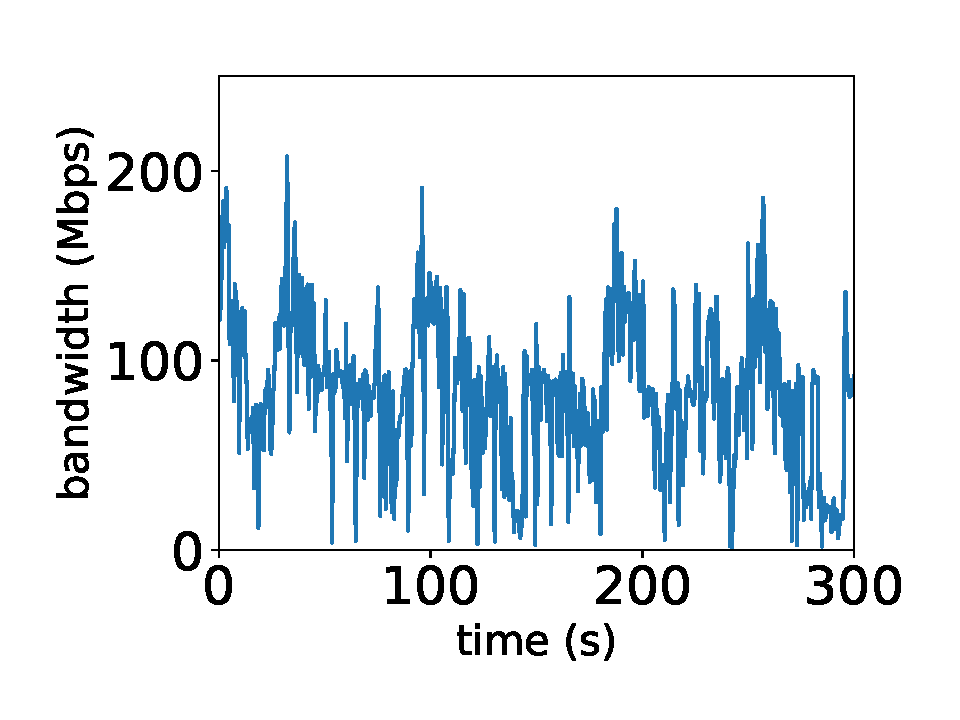
\includegraphics[width=0.48\linewidth]{fig/indoors.pdf}}
    \hfil
    \subfloat[Outdoors\label{fig:outdoors}]{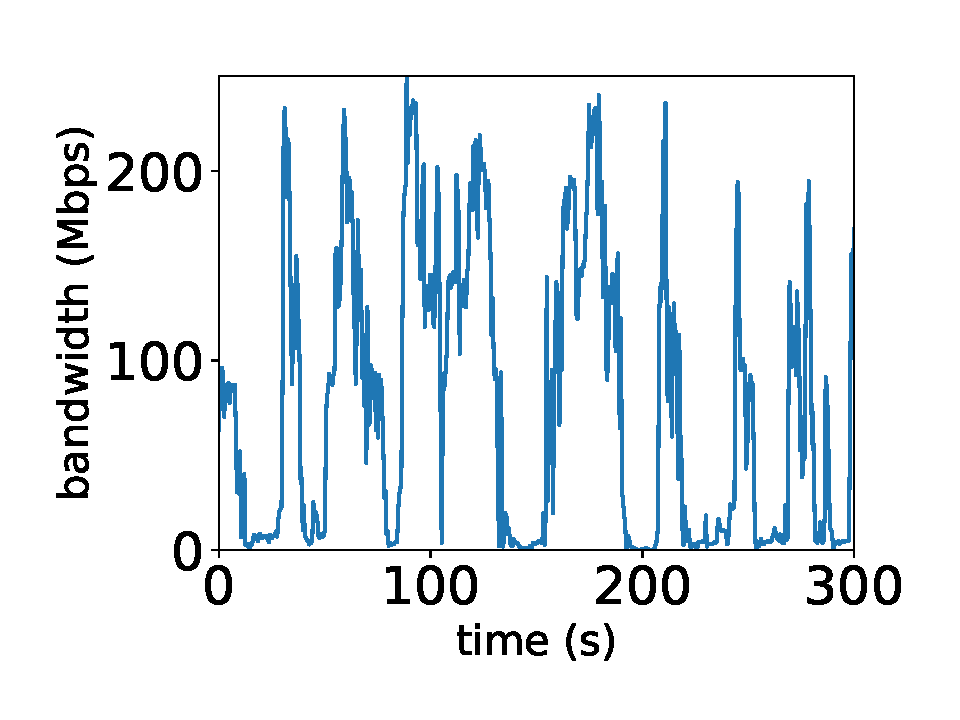
\includegraphics[width=0.48\linewidth]{fig/outdoors.pdf}}
    \caption{The instability of wireless transmission between our robot and a base station in robotic IoT networks.}
    \label{fig:bandwidth} 
\end{figure}


The results in Fig.~\ref{fig:bandwidth} show average bandwidth capacities of 93 Mbps and 73 Mbps for indoor and outdoor scenarios, respectively. 
The outdoor environment exhibited higher instability, with bandwidth frequently dropping to extremely low values around 0 Mbps, due to the lack of walls to reflect wireless signals and the presence of obstacles like trees between communicating robots, resulting in fewer received signals compared to indoor environments. This limitation on the bandwidth of robots' wireless network poses significant challenges for the efficient and reliable operation of robots in real-world scenarios, particularly in outdoor environments where the instability of wireless networks is more pronounced.

\subsection{Related Work}
Collaborative Inference expedites the overall inference process by leveraging a GPU server to handle a portion of the computational workload. 
While the DSCCS approach~\cite{liang2023dnn} focuses on model layer-level scheduling (layer partitioning) for rapid inference, Hybrid-Parallel~\cite{sun2024hybridparallel} offers a more fine-grained control by scheduling at the local operator level, enhancing parallelism and further accelerating inference. 
However, despite the advancements in Hybrid-Parallel techniques, the limited bandwidth still poses a bottleneck for data transmission, which our caching mechanism effectively mitigates, resulting in a significant improvement in inference performance.

Cache related (Guan will take it)

\section{System Overview}
% The chapter presents an overview of the architecture of CacheInf.

\subsection{Working Environment}
We assume that the working environment of CacheInf is a mobile robot performing robotic tasks in a real-world field which requires seamless real-time visual model inference on the continuous image stream captured from the on-board camera, to achieve real-time response to various environment changes.
The robot itself is equipped with low-power-consumption gpu to perform visual model inference which is slow and consumes too much power; it has wireless network access to a remote powerful GPU server that provides opportunity of acceleration, but the connection suffers from limited and unstable wireless network bandwidth.

% While the requirements of real-time inference does not necessarily imply the requirement of high inference frequency, we measure the real-time metric by the average end-to-end inference latency when the robot is seamlessly performing inference, which leads to high inference frequency; the power consumption is also measured by average power consumption to finish inference on each image in the same scenario.

\subsection{Architecture of CacheInf}
CacheInf consists of four major components: CacheInf Scheduler, Cache Tracker, Cache-Aware Collaborative Inference and Cache Recoverer.
CacheInf Scheduler functions at the initialization stage and we exclude it in Figure~\ref{fig:overview} which describes the runtime of CacheInf for simplicity.

\subsubsection{CacheInf Scheduler}
During the initialization stage of the robotic task and CacheInf is granted access to a visual model and an initial input image.
CacheInf Scheduler first profiles the visual model based on this initial input and its execution statistics on both the robot and the server.
Then it decides on the set of operators involved in the visual model that should cache their computation results and computes for an optimized computation and offloading plan for each possible situation including different wireless network bandwidth and different ratio of reusable cache.

\subsubsection{Cache Tracker}
Given a pair of consecutive image inputs and the the former one's computation intermediates at the selected operators are cached, Cache Tracker identifies the reusable portion of these computation intermediates.
We use the standard image stitching method to try to stitch as large as possible area of the two images, which results in a perspective transform that maps the pixels from the former image to the latter.
And the same perspective transform can be applied to the cached computation results since they are computed by local operators that keep the local geometries of the input image.
We then filter the difference between the mapped pixel pairs and find areas of similar appearance whose correspondent cache is reusable.
Pixels from uncached areas are finally gathered for computation.
% Given an input image, we extract and store its features using classic computation vision methods (we choose Flann algorithm in our implementation, which is state-of-the-art).
% For a current next image, we also extract and store its features and match them with the previous features (e.g., using KNN algorithm) and compute a perspective transform between the two images, which transforms the previous image such that the transformed previous image partially overlaps the current image and the non-overlapping areas are also marked.
% The features of the previous images is then discarded.
% The same transform can also be applied to the cached computation results since they are computed by local operators that keep the local geometries of the input image, and thus the reusable cached computation results are identified.
Note that the computation involved in this process is light-weight compared with the visual model inference that typically involves hundreds of operators.

\subsubsection{Cache-Aware Collaborative Inference}
In this stage, we select a precomputed plan based on the current estimated wireless network bandwidth and the estimated ratio of reusable cache and execute it.
We pass the gathered sparse pixels that need computation through the sequence of operators involved in the visual model.
When a local operator with cache is met, we gather extra pixels from cache 
When offloading is required, we slice the input into two splits at the planned ratio and assign them to the robot and the server.

We compute the gathered sparse pixels on the sequence of sparse local operators


CacheInf mainly consists of four components: 1. CacheInf Scheduler that profiles the visual model and its execution statistics on both the robot and the server and computes an optimized computation and offloading plan on various cache situations; 
2. Cache Tracker that compares the appearance of consecutive image inputs, identifies the reusable cache and extract uncached areas for computation;
3. Cache-Aware Collaborative Inference that executes the planned computation and offloading and update cache;
4. Cache Recoverer that merges the computation result on the sparse uncached areas with cache and forms correct result of the global geometry.


\begin{figure*}[!htb]
    \centering
    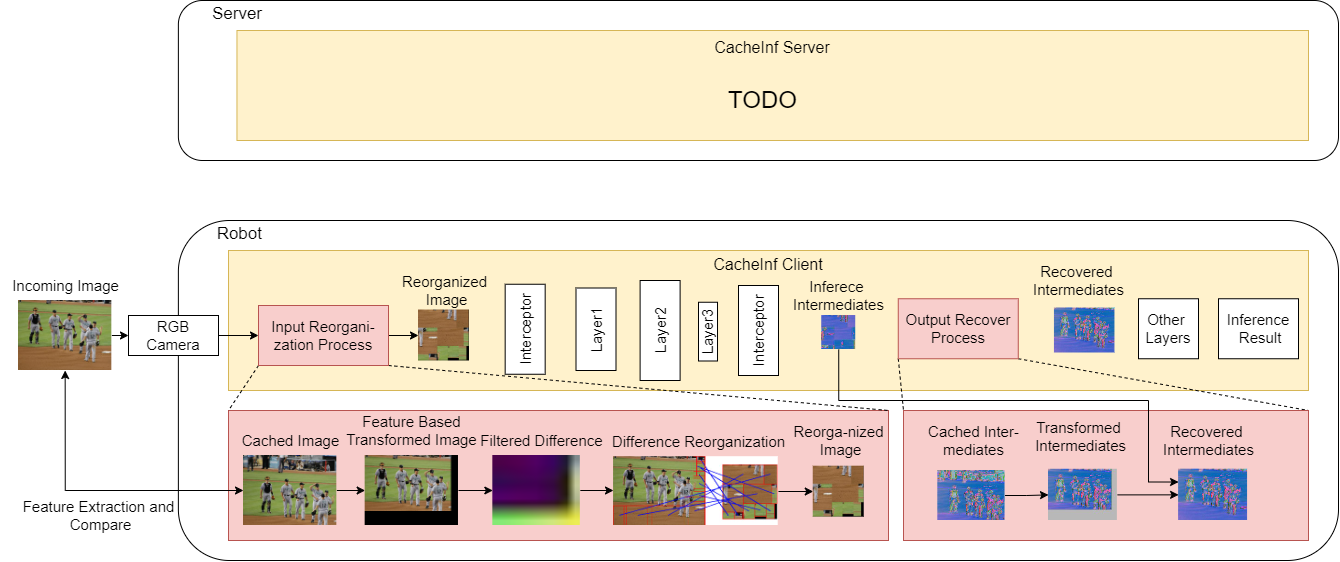
\includegraphics[width=\linewidth]{fig/overview.png}
    \caption[track]{Architecture and working process of CacheInf.}
    \label{fig:overview}
\end{figure*}

\subsubsection{Scheduler (TODO fix the names)}
During the initialization stage of the robotic task and CacheInf, CacheInf is granted access to the visual model and an initial input image and we mainly greedily pre-compute a schedule of various situations at this stage, since scheduling at runtime affects the real-time performance of the robotic task.
We first profile the model at both the robot and the remote GPU server to gather information  including shapes of the computation intermediates, the execution time of each operator (e.g., convolution, linear, etc.) on various scale of the input (e.g., from one tenth of the image to full scale of the image), the local property of each operator (i.e., whether the operator performs local computation) and so on.

Based on the above information, CacheInf finds sets of continuous local operators and assign the operators with smallest output sizes to be the operators to cache their computation results to reduce memory consumption of cache.
Then we coarsely iterate through the possible wireless network bandwidth, distribution of cache between the robot and the server and the portion of reusable cache and greedily compute a plan of whether to compute on cache and the portion of local computation and offloaded computation at the server at the reduced transmission data volume reusing cache.
We use the greedy strategy because we assume that both the wireless network bandwidth and the portion of reusable cache is unpredictable in the real-world scenario.
Note that the precomputed schedule can be reused for a same visual model with the same settings. 

\subsubsection{Cache Tracker}
At runtime, the selected operators at the previous stage will cache their computation results and the cache tracker identifies the reusable portion of such cached computation results.
Given an input image, we extract and store its features using classic computation vision methods (we choose Flann algorithm in our implementation, which is state-of-the-art).
For a current next image, we also extract and store its features and match them with the previous features (e.g., using KNN algorithm) and compute a perspective transform between the two images, which transforms the previous image such that the transformed previous image partially overlaps the current image and the non-overlapping areas are also marked.
The features of the previous images is then discarded.
The same transform can also be applied to the cached computation results since they are computed by local operators that keep the local geometries of the input image, and thus the reusable cached computation results are identified.
Note that the computation involved in this process is light-weight compared with the visual model inference that typically involves hundreds of operators.

\subsubsection{Executor (TODO fix the names)}
The executor is responsible to actually select and execute an plan based on results of the above two processes at runtime.
First, we further estimate the actual possible speedup by reusing cache, because the areas without cache needed for computation are often sparse and fragmented.
We cluster the areas without cache into different nearest clusters and compute minimum bounding boxes for each of the clusters;
then we greedily break up and recombine these bounding boxes to form a minimum new rectangle as a temporary input for the local operators and estimate its execution time based on its shape and the profile results from the initialization stage and select a precomputed plan for this input shape.
If no evident speedup, we will ignore the cache and use the whole input.

With a selected plan where cache is enabled, the executor reuses the temporary input of reorganized areas without cache described above and feed it into the inference pipeline; it also handles the portion of local computation and the portion of offloaded computation to the remote GPU server.
When appropriate, the executor breaks up the computation results of the temporary input and combines them with the transformed cache to recover geometries of the input image to get the correct result.
With a selected plan where cache is disabled, the actions with cache involved are excluded, but note that in any cases, the cache at the remote GPU server is always reused to reduce transmission data volume.











\section{Design}
% This chapter presents the detailed design for CacheInf to fulfill the functionality of tracking and reusing cached computation results and scheduling for actions among local computation, offloading or hybrid, with or without cache, to optimally reduce visual model inference latency for mobile robots.

\subsection{Cache Analyzer, Cache Combiner and Recomputation Input Constructor}
As described above, Cache Analyzer extracts the motion vectors of small pixel blocks of the input image and combines (average) the the motion vectors of small pixel blocks involved in a receptive field as the motion vector for the receptive field of the cached activations.
\begin{equation}
    \begin{aligned}
        \min\limits_{\textit{\textbf{$i,j$}}} &\enspace \frac{(P_{k,l}-P_{i+k,j+l}')^2}{n}\\
         s.t. \enspace \enspace& 0 \le k \le M \\
         & 0 \le l \le N \\
         & 0 \le i + k \le M \\
         & 0 \le j + l \le N \\
    \end{aligned}
    \label{eq:block_matching}
\end{equation}
The motion vectors can be computed as in Eq.~\ref{eq:block_matching} which is a block matching process that minimizes mean square error (MSE) between small pixels blocks in the cached input image and the new input image, where $P_{k,l}$ is a small pixel block indexed by $(k,l)$ in the cached input image and $P_{i+k,j+l}'$ is a small pixel block on the new input image with offset as $(i,j)$ and $(i,j)$ is the motion vector of $P_{k,l}$. 
Both images are of size $M*N$ and each pixel block consist of $n$ pixels.

When the above computation process finishes, we obtain the final minimized MSE of each small pixel blocks and high MSE indicates that a pixel block on the cached input image cannot finely match on the new input image, and thus we select such pixel blocks with MSE above a threshold as sparse update (compensation pixels) to the cached input image.
Inversely, Cache Combiner moves pixel blocks on the cached image and the cached activations according to the motion vectors and merge the compensation pixels to the cached image and the cached activations.

The variance of motion vectors of small pixel blocks in a receptive field (internal variance) is computed as in Eq.~\ref{design:variance}
\begin{equation}
    var_i = \frac{1}{m}\sum_j (MSE_{max} -MSE_j)\cdot (mv_j - \hat{mv})
    \label{design:variance}
\end{equation}
where the $j$ indexed small pixel block resides in the receptive field indexed by $i$. 
$MSE_{max}$ is the maximal mean square error of small pixel blocks within the receptive field and $mv_j$ and $\hat{mv}$ are motion vectors indexed by $j$ and the average motion vector of motion vectors in the receptive field.
The internal variance of a receptive field describes how the pixel blocks in this receptive field diverges in movement which distinguishes moving objects instead of stationary background captured from a moving camera and the existence of new information.
Note that the factor $(MSE_{max} -MSE_j)$ is used to filter out motion vectors caused by pixel blocks on the cached input image which cannot finely match on the new input image since these pixel blocks tend to generate random motion vectors.

With the calculated receptive field internal variance, Recomputation Input Constructor collects pixels on the updated cached input image from the receptive field with the highest internal variance and its surrounding receptive fields that meets a internal variance threshold.
The resulting sub-image will be fed to the subsequent inference pipeline.
Note that the inference process will be intercepted by Cache Combiner when the selected operator with its output activations cached, where Cache Combiner merge the computed partial activations back to the cached activations and then the subsequent calculation will be conducted on the full-sized updated cached activations.



\subsection{Collaborative Offload Scheduler}
We define the ratio of pixel blocks on the input image whose computed MSE is above a threshold (mismatched) as $c$ and we define the computation time before the cached operator as $T_r$ for the robot and $T_s$ and the execution time of the rest operators as $T_r'$ and $T_s'$. 
We suppose the size of the collected recomputation input $R$ by Recomputation Input Constructor and the transmission data volume $V$ of CacheInf metadata are both proportional to $c$, and the proportional counterparts are referred to as $R_c$ and $V_c$.
We assume $T_r$ and $T_s$ are proportional to the recomputation input size $R_c$.
The major goal of Collaborative Offload Scheduler is to statically find an optimal placement of computation for a period of given times ($n$) of inference for each pair of wireless network bandwidth $b$, $r$ and the current placement of computation $p$, supposing that the bandwidth and $r$ will hold during during the period.

\begin{algorithm}[htbp]
    \caption{\small Collaborative Offload Schedule\label{alg:schedule}}
    \SetKwInput{KwInput}{Input}                % Set the Input
    \SetKwInput{KwOutput}{Output}              % set the Output
    \DontPrintSemicolon
      \KwInput{\small Wireless network bandwidth $b$; ratio of mismatched pixel blocks $c$; current computation placement $p$; consideration period $n$}
      \KwOutput{\small The static schedule of computation placement under $b,c,p$, $schedule$}
    %   \KwData{\small input of $i_{th}$ layer $Z_{i}$; schedule plan of $i_{th}$ layer under the $b$ bandwidth $X_{i}^{b}$, $M_{i}^{b}$,$N_{i}^{b}$}
    
    $robot\_time = 0$
    
    $server\_time = 0$
    
    $r = R_c / R$


    \tcp{\footnotesize First inference time cost}
       \If{$p$ == robot}{

        $server\_time = V / b + T_s + T_s'$

        $robot\_time = T_r*r + T_r'$

       }
       \Else{
        $robot\_time = T_r + T_r'$

        $server\_time = V_c / b + T_s*r + T_s'$

        }

        \tcp{\footnotesize Subsequent inference time cost}

       $server\_time += (n-1)*(V_c / b + T_s*r + T_s')$

       $robot\_time += (n-1)*(T_r*r + T_r')$

       \If{$robot\_time > server\_time$}{
        schedule = server
       }
       \Else{schedule = robot}
      
\KwRet{$schedule$}

\end{algorithm}

As shown in Algo.~\ref{alg:schedule}, we estimate the time cost of switching the computation placement from current $p$ to either the robot and the GPU server for $n$ inference.
If the current computation placement is at the robot, switching to the GPU server will incur full transmission of the input data and full computation on the visual model (line 5); if and the GPU server side, switching to the robot will incur full computation on the visual model (line 9).
If current computation placement remains, for the robot side, each inference incurs time cost of visual model inference proportional to $c$ (line 6 and 13) and for the server side, each inference incurs time cost of both transmission and visual model inference (line 10 and 12).
Finally we select the computation placement with least estimated inference time for $n$ inference as the scheduled computation placement.

Note that the above process is conducted offline during the system initialization stage.
At runtime, as the robot collects the input images and estimates the wireless network bandwidth, Collaborative Offload Scheduler maintains an estimation of $b$ and $c$ and every $n$ inference update the computation placement by querying the precomputed schedule.
Computation placement to either the robot or the GPU server will cause the CacheInf metadata computed by the previous stages to be transmitted to either the CacheInf Executor at the robot side or at the GPU server side for inference result computation.
If the placement is at the GPU server side, the inference results will be transmitted back to the robot as show in Fig.~\ref{fig:overview}.


% \subsection{Identifying Reusable Computation Results\label{sec:reusable cache}}
% To find and match similar local geometries between consecutive images in a stream of images $\textit{\textbf{I}}=\{I_1, I_2, ..., I_n\}$ to identify reusable cache, we use the standard image stitching procedure: given a pair of consecutive images $I_j$ and $I_{j+1}$, their key points and key point descriptors (or feature vectors) are computed and matched within a distance threshold of the feature vectors; then a homography matrix $M$ is computed based on the corresponding relationship between the key points on each image which minimizes the error.
% The resulting homography matrix is then used to apply perspective transformation to each pixel in $I_j$ to form a new image $\hat{I}_{j+1}$ closest to $I_{j+1}$ as shown in Equation~\ref{eq: pt}, where $(u_j,v_j)$ and $(\hat{u}_{j+1},\hat{v}_{j+1})$ and pixel indices on $I_j$ and $\hat{I}_{j+1}$.
% It is also depicted in the Feature Based Transformed Image in Fig.~\ref{fig:overview}.
% Since the computation of local operators relies on local geometries, the same transformation can be applied to intermediate computation results of the following local operators.
% \begin{equation}
%     (\hat{u}_{j+1},\hat{v}_{j+1},1) = M \times (u_j,v_j,1)
%     \label{eq: pt}
% \end{equation}

% While the above process minimizes error between $\hat{I}_{j+1}$ and $I_{j+1}$, the remaining different areas between them are the areas of new information which are uncached and need to be recomputed.
% We filter and identify these areas by applying average pooling over the difference between $\hat{I}_{j+1}$ and $I_{j+1}$ and the pixels with computed difference greater than a preset threshold $N$ (default to be 0.1 when we normalize the value of each  channel of a pixel to between 0 and 1) will be marked as needed to be recomputed as in Equation~\ref{eq:avg_pool}, where $u,v$ are the pixel indices.

% \begin{equation}
%     \textit{\textbf{uv}} = \{(u,v)|AveragePooling(|\hat{I}_{j+1} - I_{j+1}|)^{u,v} \geq N\}
%     \label{eq:avg_pool}
% \end{equation}

% Suppose there are $Q$ pixels in \textit{\textbf{uv}} and $H$x$W$ total pixels in each image,
% we define the cache ratio between $I_j$ and $I_{j+1}$ as $r = \frac{Q}{H\cdot W}$.

% \subsection{Sparse Local Operators\label{sec:sparse}}
% From the above discussion, we have identified the pixels needed to recompute \textit{\textbf{uv}} and we suppose their corresponding features $f_{inp}$ are of size $B$x$C_1$x$Q$, along with the cached input defined as $I'_{inp}$ of size $B$x$C_1$x$H$x$W$.
% Now we focus on how to compute the correct results based \textit{\textbf{uv}}, $f_{inp}$ and $I'_{inp}$.
% There are mainly two kinds of local operators: element-wise local operators such as addition, subtraction, multiplication and division, which solely depends on the value of each element; and convolution local operators such as convolution, average pooling and max pooling, which is influenced by the surrounding areas (e.g., a 2D kernel) of each element .
% We mainly focus on the latter type of local operators since the element-wise local operators can be viewed as a special case of convolution local operators where the surrounding area is of size one.

% We first consider the scenario with dense input.
% Assume an image (or feature map) $I_{inp}$ of size $B$x$C_1$x$H$x$W$, a convolution local operator $K$ with its kernel sized $C_2$x$C_1$x$K_1$x$K_2$, stride 1 and no padding and its output feature map $I_{out}$ of size $B$x$C_2$x$H'$x$W'$, then each of the value of the output feature map is determined by
% \begin{equation}
%     I_{out}^{i,j,k,l} = \sum_{c=1}^{C_1} \sum_{m=1}^{K_1} \sum_{n=1}^{K_2} K^{j,c,m,n} * I_{inp}^{i,c,k+m-1,l+n-1}, 
%     \label{eq:kernel}
% \end{equation}
% Omitting the batch dimension and the channel dimension (first two dimension) of $I_{out}$, we can learn from Equation~\ref{eq:kernel} that an output value is determined by an area of $K_1$x$K_2$ on $I_{inp}$ and we define pixels in this area as
% \begin{equation}
%     P_{k,l} = \{(u,v)|k\leq u < k+K_1 \land l\leq v < l+K_2\}
%     \label{eq:set}
% \end{equation}
% where $(k,l)$ is the pixels indices on $I_{out}$.

% Moving to the sparse scenario, 
% the indices of pixels on $I_{out}$ that have updated value with \textit{\textbf{uv}} as input would be 
% \begin{equation}
% \textit{\textbf{uv}}' = \{(k,l)|\exists P_{k,l}, s.t. P_{k,l}\cap \textit{\textbf{uv}} \neq \emptyset\}
% \end{equation} 
% which can be view as wrapping around pixels in \textit{\textbf{uv}} by $K_1$x$K_2$ and may involve pixels in $I'_{inp}$.

% Note that $\textit{\textbf{uv}}$ and cached input $I'_{inp}$ are possibly in different planes determined by the homography matrix $M$.
% We may transform the cached intermediates every time before computation, but it will unfortunately involve computation of the whole feature map and invalidate the acceleration of sparse computation.
% Instead, during computation we query the original cached intermediates by transforming the pixel indices with $M$:
% \begin{equation}
%     F(i,j,u,v, I'_{inp}, f_{inp}) = \left\{
%         \begin{aligned}
%             f_{inp}^{i,j,u,v}  & , & (u,v) \in \textit{\textbf{uv}}, \\
%             {I'}_{inp}^{i,j,G(u,v,M)} &, & (u,v) \notin \textit{\textbf{uv}}
%         \end{aligned}
%         \right. 
%     \label{eq:query}
% \end{equation}
% where $G(u,v,M) = H^{-1}(M^{-1}\times H((u,v)))$ which transforms $(u,v)$ into the plane of cached input $I'_{inp}$, and $H(\cdot)$ and $H^{-1}(\cdot)$ means turning a vector to a homogeneous vectors and the opposite.
% Then for $(u,v)\in\textit{\textbf{uv}}'$, the corresponding computed output is
% \begin{equation}
%     f_{out}^{i,j,u,v} = \sum_{c=1}^{C_1} \sum_{m=1}^{K_1} \sum_{n=1}^{K_2} K^{j,c,m,n}\cdot F(i,c,k+m-1,l+n-1, I'_{inp}, f_{inp})
% \end{equation}
% Until now we get the indices of the altered output values in output feature map $\textit{\textbf{uv}}'$ and the corresponding features $f_{out}$ which can then be passed to the subsequent computation.

% Along the local operators where local geometries are preserved, we can repeat the above process by passing only the sparse features and their indices and do not need to merge the sparse features with cache.
% When a non-local operator is met (e.g., matrix multiplication), we transform its cached input with $M$ and merge $f_{inp}$ into the transformed input according to their sparse indices $\textit{\textbf{uv}}$, which recovers the correct geometries of the whole feature map.
% To minimize performance impact to update $I'_{inp}$, we update $I'_{inp}$ by transforming $I'_{inp}$ and merge it with $f_{inp}$ only after the whole computation process finishes, when the system is typically idle and waiting for the next input.

% Also, to save memory consumption of cached intermediates, notice that the above process is basically wrapping the sparse pixels with the kernel size $K_1$x$K_2$ and computing on the wrapped pixels, we can merge the query process in Equation~\ref{eq:query} of multiple convolution local operators into the first convolution local operator.
% For example, if a next operator is a convolution local operator with kernel size $K'_1$x$K'_2$, we can wrap the sparse pixels with an extended kernel size $(K_1+K'_1)$x$(K_2+K'_2)$ in the first local operator, and the wrapping process of the next operator is skipped (we refer to this process as merging cache).
% In this case, the cache for the input of the next operator is needless and can be excluded to save memory consumption and the reduced number of cached input further leverages the cost to update $I'_{inp}$.


% % In the above discussion we have analyzed the opportunity for visual model inference acceleration by reusing previous computation result.
% % In a edge-cloud collaborative system as CacheInf, reusing previous computation result has the potential to not only reduce transmission time by reducing transmission data volume, but also reduce local computation time by shrinking computation size using sparse local operators, and the extend of such reduction is determined by cache ratio of the current input $r$.
% We define all the operators involved in a visual model as $\textit{\textbf{O}} = \{o_1, o_2,...,o_n\}$ and the portion of locally executed input of each operator as $\textit{\textbf{X}}=\{x_1, x_2, ..., x_n\}$, $0\le x_i \le 1$ and $1-x_i$ represents the the portion of input executed on the GPU server.
% The indices of local operators is defined as $\textit{\textbf{O}}_l$.
% While offloading, we transmit the sparse features together with their indices encoded as a bit-mask and the transmission volume is almost inversely proportional to cache ratio $r$.
% % : assume wholely offloading computation of a visual model from a layer will require transmission of $m=B$x$C$x$H$x$W$ element and each element is a float32 number, summing up to 4m bytes data; in the cached case with cache ratio $r$, the data volume needed to transmit will be $(1-r)4m + \frac{m}{8BxC}$ bytes, where the latter term is the bit-mask of $H$x$W$ encoding the indices of the transmitted pixels on the whole feature map.
% % When integrating Hybrid-Parallel that would slice the sparse features, we simply slice the sparse features and only encode the bit-mask for indices of the slice for the server, while preserving the features and indices for the robot.

% However, the local computation time acceleration with sparse local operators has a complex relationship with cache ratio, which is affected by the operator implementation, gpu structure and so on.
% Thus we profile such relationship by altering the cache ratio and $x_i$ and record the average execution time for every operator involved in the visual model and we define the profile result as a function $T_c(o_i, x_i, r)$ for the robot ($c$ means client) and $T_s(o_i, x_i, r)$ for the server, which returns the execution time of operator $o_i$ under $x_i$ with cache ratio $r$.
% We also profile the time cost to update cached input for each local operator and get $U_r(o_i, x_i, r)$ and $U_s(o_i, x_i, r)$.
% Note that for non-local operators ($\textit{\textbf{O}}_{nonlocal}=\{i|1\le i\le n \land i \notin \textit{\textbf{O}}_l\}$), we make both $T(\cdot)$ and $U(\cdot)$ returns time of computation on the whole input.

% \subsubsection{Schedule to Merge Cache}
% With the above setup, the first problem to solve will be the choices of merging the cache of sparse local operators to further accelerate computation while saving memory consumption.
% We define the indices of the chosen operators to cache their input as $\hat{\textit{\textbf{O}}}_c$ and the resulting reduction of cache ratio (since extra input will be included) of each operator as $o_I$ to be $R(\hat{\textit{\textbf{O}}}_c, o_i)$.
% Since these choices will determine the operators that will cache their input and will be reused across different inference, these choices should be fixed during the whole inference task.
% Thus we start by considering only the worst case where offloading is not possible and $\forall x_i\in \textit{\textbf{X}}, x_i=1$.
% In this case the execution time of every operator will be $T_c(o_i, 1, r-R(\hat{\textit{\textbf{O}}}_c, o_i))$, and the optimization problem will be 
% \begin{equation}
%     \min\limits_{\hat{\textit{\textbf{O}}}_c \subset \textit{\textbf{O}}_l} \frac{1}{w} \sum_{i=1}^n \sum_{j=0}^w T_c(o_i, 1, r_j+R(\hat{\textit{\textbf{O}}}_c, o_i)) + U_{sum}(\hat{\textit{\textbf{O}}}_c, r_j)
%     \label{eq:cached op}
% \end{equation}
% where $r_j = \frac{j}{w}$ with $w>1$ is the possible cache ratio considered (we empirically set $w$ to 10), and $U_{sum}(\hat{\textit{\textbf{O}}}_c, r) = \sum\limits_{k \in \hat{\textit{\textbf{O}}}_c} U(o_k, x_k, r)$ is the total time to update cache of operators in $\hat{\textit{\textbf{O}}}_c$.

% Solving of this optimization problem seeks the optimal choices of cache operators $\hat{\textit{\textbf{O}}}_c$ that minimizes local execution time averaged across all possible cache ratio.
% Note that we do not need to explicitly consider memory consumption because the latter term in Equation~\ref{eq:cached op} will naturally reduce the number of cached operators and favor operators with smaller size of input and thus shorter time to update cache.

\subsection{End-to-End Runtime\label{sec:schedule}}
Finally, we are combining all the above components to schedule for computation and offloading in a cache-aware way to optimize end-to-end inference latency for robotic visual models.
With Hybrid-Parallel integrated, cache can exists partially both at the robot and the server and we analyze the cache ratio on robot $r_c$ and the cache ratio $r_s$ on server by enquiry the current cached pixels with the previous slice of input (i.e., $x_i$).
For an $x_i$, we define the minimum portion of locally executed input of its parent operators (i.e., operators whose output is the input of $o_i$) as $x'_i$ and different between $x_i$ indicates offloading to/from the server.
For every operator $o_i \in \textit{\textbf{O}}$ involved in a visual model, we define its finishing time since the first operator starts executing as $t_i^{c}$ on the robot ($c$ means client) and $t_i^{s}$ on server.

We can have the finish time of each operator on the robot and the server as the following, where $D(o_i, x'_i-x_i,r)$ is the data volume needed to be transmitted at operator $o_i$ with cache ratios $r_c$ and $r_s$ and $b$ is the estimated bandwidth:
\begin{equation*}
    t_i^{c} = \left\{
        \begin{aligned}
            &t_{i-1}^{c} + T_c(o_i, x_i, r_c-R(\hat{\textit{\textbf{O}}}_c, o_i)),&&1\le i\le n \land x_i\le x'_i \\
            &max(T_c(o_i, x_i, r_c-R(\hat{\textit{\textbf{O}}}_c, o_i)) +\\
            & \enspace \enspace t_{i-1}^{c}, \enspace \frac{1}{b}D(o_i, x'_i-x_i,r)+ t_i^{s}),&&1\le i\le n \land x_i >x'_i
        \end{aligned}
    \right.
\end{equation*}

\begin{equation*}
    t_i^{s} = \left\{
        \begin{aligned}
            &t_{i-1}^{s} + T_s(o_i, 1-x_i, r_s-R(\hat{\textit{\textbf{O}}}_c, o_i)),&&1\le i\le n \land x_i\ge x'_i \\
            &max(T_s(o_i, 1-x_i, r_s-R(\hat{\textit{\textbf{O}}}_c, o_i)) + \\
            & \enspace \enspace t_{i-1}^{s}, \enspace \frac{1}{b} D(o_i, x'_i-x_i,r_s)+ t_i^{c}),&&1\le i\le n \land x_i<x'_i
        \end{aligned}
    \right.
\end{equation*}
The first rows of the above two equations describe the scenarios where either the robot or the server does not need to receive data from the opposite side and thus the finishing time of this operator only depends on its local execution time.
The second rows instead describe the opposite scenarios, where either the robot or the server needs to receive data from the opposite side (e.g., $x_i > x'_i$ for the robot) and have to wait until the same operator to finish computing at the opposite side and then be transmitted at bandwidth $b$.

With the above statements, optimizing the end-to-end inference latency for the visual model with cache enabled at a given bandwidth $b$ and cache ratios $r_c$ and $r_s$ is to solve
\begin{equation}
    \begin{aligned}
        \min\limits_{\textit{\textbf{X}}} & t_n^{c} \\
         s.t. \enspace \enspace&  x_1 = x_n = 1 \\
         & \forall j \in \textit{\textbf{O}}_{nonlocal}, x_j (mod \enspace 1) = 0 \\
         & \forall j \notin \hat{\textit{\textbf{O}}}_c, x_j = x'_j
    \end{aligned}
    \label{eq:e2e}
\end{equation}
In Equation~\ref{eq:e2e}, the first two constraints ensure that inference output will finally be located at the robot and non-local operators will always have full input; the third constraint ensures that offloading will not happen within an operator whose cached is merged into the cache of other operators, since we cannot recover the operator's whole feature map.
% We solve both optimization problems in Equation~\ref{eq:cached op} and~\ref{eq:e2e} with the differential evolution algorithm~\cite{qin2008differential} and store the solutions of different bandwidth and cache ratios of Equation~\ref{eq:e2e} in a dictionary referred to as $Schedule$.

The resulting algorithms of CacheInf at both the robot and the server are presented in Algorithm~\ref{alg:client} and Algorithm~\ref{alg:server}.
Line 1 to 3 in Algorithm~\ref{alg:client} and Line 1 to 4 in Algorithm~\ref{alg:server} profile the model at both the robot and the server and compute a schedule as described in Section~\ref{sec:schedule}, where the computation is located on the server to speed up computation.
The rest of Algorithm~\ref{alg:server} is basically mirrored from that of Algorithm~\ref{alg:client} and thus we focus on Algorithm~\ref{alg:client} for simplicity.

\begin{algorithm}[htbp]
    \caption{\small CacheInfClient\label{alg:client}}
    \SetKwInput{KwInput}{Input}                % Set the Input
    \SetKwInput{KwOutput}{Output}              % set the Output
    \DontPrintSemicolon
      \KwInput{\small A continual sequence of video images $\textit{\textbf{I}}$; DNN model $M$}
      \KwOutput{\small The inference results $ret$ on each image in $\textit{\textbf{I}}$ }
    %   \KwData{\small input of $i_{th}$ layer $Z_{i}$; schedule plan of $i_{th}$ layer under the $b$ bandwidth $X_{i}^{b}$, $M_{i}^{b}$,$N_{i}^{b}$}
       \tcp{\footnotesize profile}
    
        $T_c, U_c = Profile(M)$
    
        $Send(M, T_c, U_c)$
    
        $Schedule, \hat{\textit{\textbf{O}}}_c = Receive()$

        $Cache = InitCache(\hat{\textit{\textbf{O}}}_c)$

       \tcp{\footnotesize inference}

       \ForEach{$I \enspace in \enspace \textit{\textbf{I}}$ \enspace}{
            $b = EstimateBandwidth()$

            $r_c, r_s = AnalyzeCacheRatio(I, Cache[1])$

            $inp, M = IdentifyCache(I, Cache[1])$

            $ Send(b, r_c, r_s, M) $

            $x, x' = Schedule[b,r_c,r_s]$

            \ForEach{$i = 1, 2, ..., n $ \enspace}{
                \If{$i \in \textit{\textbf{O}}_{nonlocal}$ and $x_i>0$ and IsSparse(inp)}{
                    $inp = DenseRecover(inp, Cache[i],M)$

                    $UpdateCache(Cache[i], inp, M)$
                }
                \ElseIf{$x'_i>0$ and $i\in \hat{\textit{\textbf{O}}}_c$}{
                    $inp = SparseGather(inp, Cache[i], M)$
    
                    $UpdateCache(Cache[i], inp, M)$
                }
                \If{$x_i < x'_i$}{
                    $inp, inp' = Slice(inp, x_i, x'_i)$

                    $Send(inp')$
                }
                \ElseIf{$x_i > x'_i$}{
                    $inp = Merge(inp, Receive())$
                }
                \If{$x_i>0$}{
                    \If{$IsSparse(inp)$}{
                        $inp = SparseExecute(o_i, inp)$ 
                    }
                    \Else{
                        $inp = Execute(o_i, inp)$
                    }
                }

            }
            $ret[I] = inp$
       }
      
\KwRet{$ret$}

\end{algorithm}


Line 6 to 8 in Algorithm~\ref{alg:client} identifies the reusable cache by matching features between the input image $I$ and its cached counterpart $Cache[1]$ and gets the homography matrix $M$ and the sparse uncached input that needs to be recomputed.
After communicating info of bandwidth, cache ratio and homography matrix with the server, we query the $Schedule$ to get input ratio $x$ and parent operator input ratio $x'$ as described in Section~\ref{sec:schedule}.
The we start executing each operator $o_i$ involved in the model sequentially.
We recover the whole input by combining sparse input $inp$ with cache for non-local operators or gather extra pixels from cache for $inp$ for sparse local operator computation at cached operators at line 12 to 19.
When offloading is required to accelerate inference, we send a slice of $inp$ to the server or merge received partial input from the server to $inp$ at line 20 to 26.
When $inp$ is finally ready and not empty, we execute the operator $o_i$ with inp where we choose the sparse local operator for sparse input and choose the original operator for dense input at line 27 to 34.


\begin{algorithm}[htbp]
    \caption{\small CacheInfServer\label{alg:server}}
    % \SetKwInput{KwInput}{Input}                % Set the Input
    % \SetKwInput{KwOutput}{Output}              % set the Output
    % \DontPrintSemicolon
    %   \KwInput{\small A continual sequence of video images $\textit{\textbf{I}}$; DNN model $M$}
    %   \KwOutput{\small The inference results $ret$ on each image in $\textit{\textbf{I}}$ }
    % %   \KwData{\small input of $i_{th}$ layer $Z_{i}$; schedule plan of $i_{th}$ layer under the $b$ bandwidth $X_{i}^{b}$, $M_{i}^{b}$,$N_{i}^{b}$}
       \tcp{\footnotesize profile and compute schedule at the server}
    
        $ M,T_c, U_c = Receive()$

        $T_s, U_s = Profile(M)$

        $Schedule, \hat{\textit{\textbf{O}}}_c = ComputeSchedule(T_s, U_s, T_c, U_c)$

        $ Send(Schedule, \hat{\textit{\textbf{O}}}_c) $

        $Cache = InitCache(\hat{\textit{\textbf{O}}}_c)$

       \tcp{\footnotesize inference}

        \While{True}{
            $ b, r_c, r_s, M = Receive()$ 

            $x, x' = Schedule[b,r_c,r_s]$

            \ForEach{$i = 1, 2, ..., n $ \enspace}{
                \If{$i \in \textit{\textbf{O}}_{nonlocal}$ and $x_i<1$ and IsSparse(inp)}{
                    $inp = DenseRecover(inp, Cache[i],M)$

                    $UpdateCache(Cache[i], inp, M)$
                }
                \ElseIf{$x'_i<1$ and $i\in \hat{\textit{\textbf{O}}}_c$}{
                    $inp = SparseGather(inp, Cache[i], M)$

                    $UpdateCache(Cache[i], inp, M)$
                }
                \If{$x_i > x'_i$}{
                    $inp, inp' = Slice(inp, x_i, x'_i)$

                    $Send(inp')$
                }
                \ElseIf{$x_i < x'_i$}{
                    $inp = Merge(inp, Receive())$
                }

                \If{$x_i < 1$}{
                    \If{$IsSparse(inp)$}{
                        $inp = SparseExecute(o_i, inp)$ 
                    }
                    \Else{$inp = Execute(o_i, inp)$ }
                }

            }
       }
\end{algorithm}
    
    
% \begin{algorithm}[htbp]
% \caption{\small CacheInfServer\label{alg:server}}
% \SetKwInput{KwInput}{Input}                % Set the Input
% \SetKwInput{KwOutput}{Output}              % set the Output
% \DontPrintSemicolon
%     \KwData{\small input of $i_{th}$ layer $Z_{i}$; schedule plan of $i_{th}$ layer under the $b$ bandwidth $Y_{i}^{b}$, $M_{i}^{b}$,$N_{i}^{b}$}
%     \tcp{\footnotesize profile phase on server}    
%     $model,info\_robot = ReceiveFromClient()$    
%     $info\_server = ProfileModel(model)$    
%     $X, Y, M, N = LOSS(info\_robot,info\_server)$    
%     $SendToClient(X,M,N)$    
%     \tcp{\footnotesize inference phase on robot}    
%     $b = PredictsBandwidth()$    
%     $Z_{0} = \emptyset$    
%     \ForEach {$i_{th} \quad layer \quad in\quad model$ }{    
%     \If{$M_{i}^{b} \neq \emptyset$}
%     {    
%     $SendToClient(Z_{i}, M_{i}^{b})$        
%     }    
%     \If{$N_{i}^{b} \neq \emptyset$}
%     {      
%     $Z_{i} = combine(Z_{i}, ReceiveFromClient())$        
%     }    
%         \If{$Y_{i}^{b} \neq \emptyset$ and $Z_{i} \neq \emptyset$}
%     {    
%         $Z_{i+1} = compute(Z_{i},Y_{i}^{b})$        
%     }
%     \Else{    
%     $Z_{i+1} = \emptyset$
%     }    
%     }       
% \end{algorithm}







\section{Implementation}
We implemented CacheInf with python, pytorch~\cite{paszke2017automatic} and taichi~\cite{taichi} on Ubuntu20.04.
The communication library used is the distributed module~\cite{torch_distributed} of pytorch with mpi backend.
We compiled pytorch with cuda-aware mpi enabled so that the mpi backend can directly read and write to cuda buffer to minimize communication overhead.
We use mpi backend instead of the popular nccl backend because nccl is unavailable on the Jetson robot we used due to structural limitation~\cite{noauthor_can_2022}.

The sparse local operators were implemented based on the bitmasked sparse nodes in taichi~\cite{taichi}, which efficiently manages the sparse pixels in a grid and preserves the spatial structure of the sparse pixels by organizing the them in a tree structure. 
With the spatial structure preserved, common optimization methods for cuda operators based on computation locality such as block shared memory~\cite{noauthor_using_2013} can be introduced to accelerate computation; our implemented sparse local operators achieved comparable performance with the original pytorch operators with the same input size.


\section{Evaluation}
\subsection{Evaluation Settings}

\begin{figure}[!t]
    \centering
    \subfloat[Four-wheeled robot]{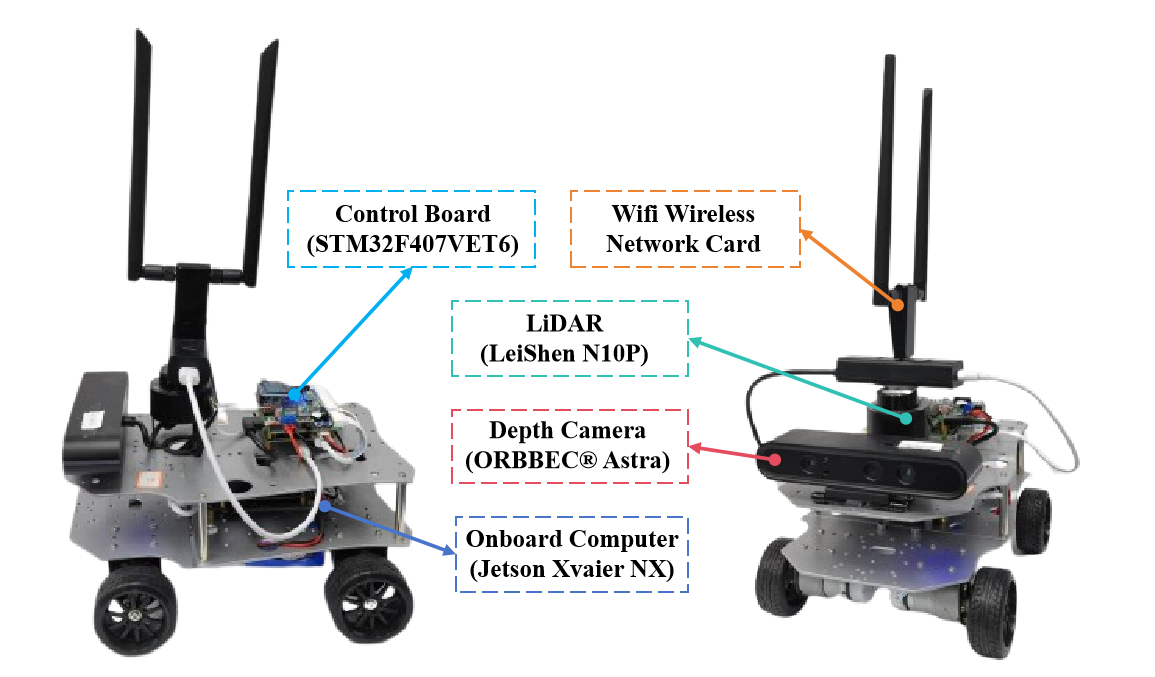
\includegraphics[width=0.48\linewidth]{fig/robot.png}\label{fig:robot}}
    \hfil
    \subfloat[Air-ground robot]{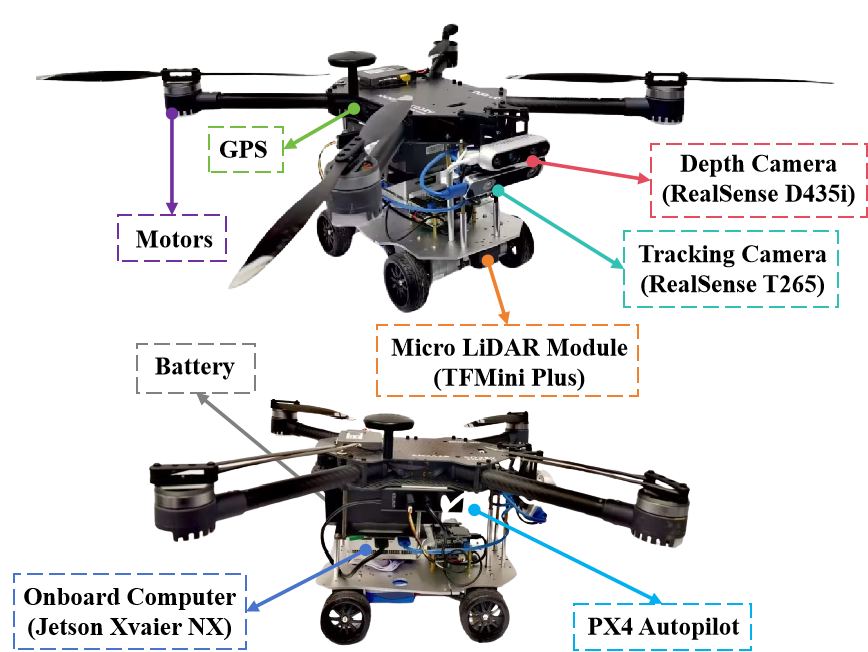
\includegraphics[width=0.40\linewidth]{fig/agr_robot.png}\label{fig:agr}}
    \vspace{-0.3cm}
    \caption{The composition of the four-wheeled robot and the air-ground robot used in our evaluation.}
    % \label{fig:robot}
    \vspace{-0.3cm}
\end{figure}

\myparagraph{Testbed}
We conducted experiments on a four-wheeled robot (Fig~\ref{fig:robot}) and a air-ground robot(Fig~\ref{fig:agr}).
Both robots are equipped with a Jetson Xavier NX~\cite{jetsonnx} 8G onboard computer with cuda acceleration capability and a MediaTek MT76x2U USB wireless network interface card for wireless connectivity.
The Jetson Xavier NX is connected to a Leishen N10P LiDAR, an ORBBEC Astra depth camera and an STM32F407VET6 controller via USB serial ports, which are managed and driven using ROS Noetic. 
The GPU server used in our experiments is equipped with an Intel(R) i5 12400f CPU @ 4.40GHz and an NVIDIA GeForce GTX 2080 Ti 11GB GPU, connected to our robot via Wi-Fi 6 over 80MHz channel at 5GHz frequency.

% Tab.~\ref{tab:energydefault} presents the overall on-board energy consumption (excluding motor energy consumption for robot movement) of the robot in various states: inference (model inference with full GPU utilization, including CPU and GPU energy consumption), transmission (communication with the GPU server, including wireless network card energy consumption), and standby (robot has no tasks to execute).
% Notice that different models, due to varying numbers of parameters, exhibit distinct GPU utilization rates and power consumption during inference. 

% \begin{table}[!t]
%     \centering
%     \begin{tabular}{|c|c|c|c|}
%     \hline
%             & inference & transmission & standby \\ \hline
%     Power (W) &     13.35        &       4.25        &    4.04   \\ \hline
%     \end{tabular}
%     \caption{Power consumption (Watt) of our robot in different states.}
%     \label{tab:energydefault}
%     \end{table}

\myparagraph{Workload}
We chose two real-world visual robotic applications as our major workloads: 1. Kapao~\cite{kapao} depicted in Figure~\ref{fig:kapao}, a RGB-image-based real-time people key point detection applications used to guide our four-wheeled robot to track and follow a walking people;
2. AGRNav~\cite{agrnav} depicted in Figure~\ref{fig:agr}, an autonomous air-ground robot navigation application that predicts unobserved obstacles by semantic prediction on point clouds and optimizes the navigation trajectory for the air-ground robot.
% We evaluated two typical real-world robotic applications on our testbed: Kapao, a real-time people-tracking application on our four-wheeled robot (Fig~\ref{fig:kapao}), and AGRNav, an autonomous navigation application on our air-ground robot (Fig~\ref{fig:agrnav}). 
% These applications feature different model input and output size patterns: Kapao takes RGB images as input and outputs key points of small data volume. In contrast, AGRNav takes point clouds as input and outputs predicted point clouds and semantics of similar data volume as input, implying that AGRNav needs to transmit more data during distributed inference. 
We also verified CacheInf's performance on a broader range of visual models common to mobile devices: VGGNet~\cite{simonyan2015deep}, ConvNeXt~\cite{woo2023convnext}, RegNet~\cite{xu2022regnet}, and we used their default implementation of torchvision~\cite{noauthor_torchvision_nodate}. 
% And we have verified several models common to mobile devices on a larger scale to further corroborate our observations and findings: DenseNet~\cite{huang2018densely}, VGGNet~\cite{simonyan2015deep}, ConvNeXt~\cite{woo2023convnext}, RegNet~\cite{xu2022regnet}.
% The models' running statistics are listed in Tab.~\ref{tab:all_app}.

\myparagraph{Dataset}
For AGRNav we used the officially available sequence of point clouds input~\cite{agrnav} and for Kapao, we used the Collective Activity Dataset (CAD)~\cite{Choi_VSWS_2009} which are sequences of video images of people doing different activities captured using hand-held cameras.
For the rest of the models from torchvision, we used the DAVIS~\cite{Perazzi2016} dataset which are sequences of video images of different objectives captured also using hand-held cameras.

\myparagraph{Experiment Environments}
The experiments across all systems and all workloads were conducted in two different real-world environments: 1. indoors, where the robot was moving in our office with desks and separators interfering wireless bandwidth;
2. outdoors, where the robot was moving in a garden with trees and bushes interfering with wireless signals and less reflection, resulting in lower bandwidth. 
The bandwidth fluctuation of each of the environments are shown in Fig.~\ref{fig:bandwidth}.
% We evaluated two real-world environments: indoors (robots move in our laboratory with desks and separators interfering with wireless signals) and outdoors (robots move in our campus garden with trees and bushes interfering with wireless signals, resulting in lower bandwidth). 

\myparagraph{Baselines}
We selected two SOTA inference acceleration methods as baselines: DSCCS~\cite{liang2023dnn} (referred to as DS), which searches for optimal layer partition strategy of a visual model to offload layers to the GPU server to accelerate inference, and Hybrid-Parallel ~\cite{sun2024hybridparallel} (referred to as HP), which enables parallelization of local computation and offloading by also partitioning the layer input / output of local operators besides layer partitioning to further accelerate inference. 
We also combined DSCCS with our cache mechanism (referred to as DS-C) to present another perspective about CacheInf's performance gain.
We refer to CacheInf as Ours in the tables.
Each result in the tables is followed with standard deviation ($\pm n$).

The evaluation questions are as follows:
\begin{itemize}
    \item RQ1: How much does CacheInf benefit real-world robotic applications by reducing inference time and energy consumption?
    \item RQ2: How does CacheInf perform on more models common to mobile devices?
    \item RQ3: How is the above gain achieved in CacheInf and what affects it?
    \item RQ4: What are the limitations and potentials of CacheInf?
\end{itemize}

\begin{figure}[!t]
    % \vspace{-0.3cm}
    \centering
    \subfloat[Targeted people]{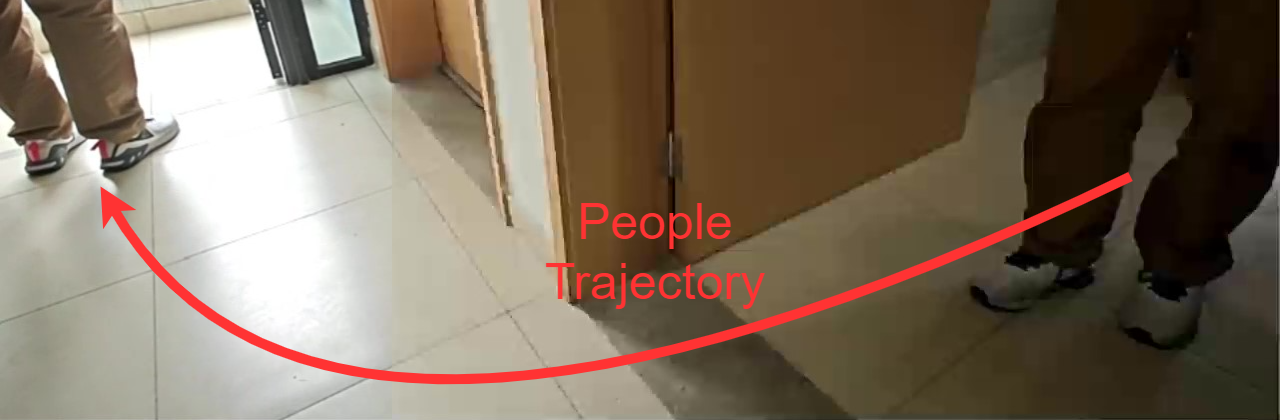
\includegraphics[width=0.95\linewidth]{fig/people.drawio.png}}

    % \vspace{-0.2cm}
    \subfloat[Robot moving trajectory]{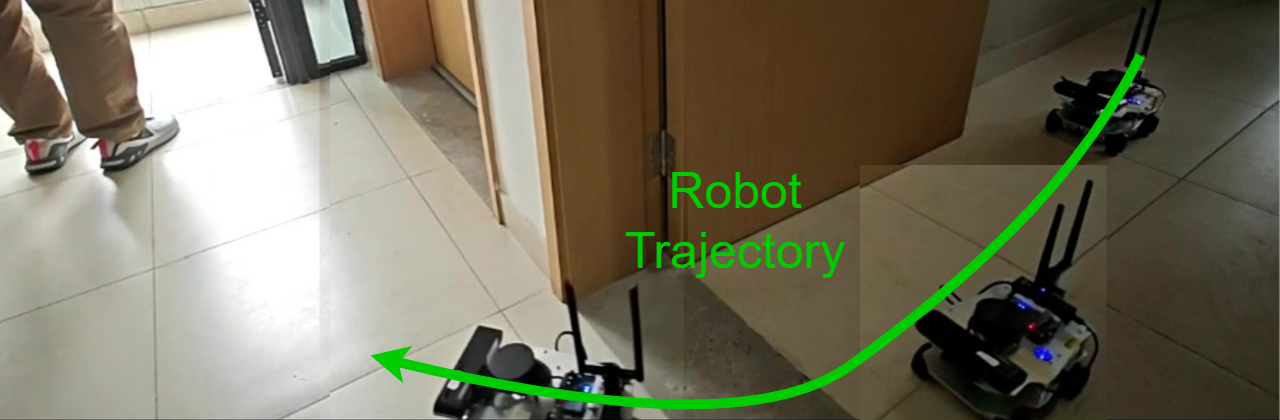
\includegraphics[width=0.95\linewidth]{fig/robot.drawio.png}}
    % \vspace{-0.3cm}
    \caption{A real-time people-tracking robotic application on our robot based on a state-of-the-art human pose estimation visual model, Kapao~\cite{kapao}.}
    \label{fig:kapao}
    % \vspace{-0.3cm}
\end{figure}

\begin{figure}[!t]
    
    % \vspace{-0.3cm}
    \centering
    \subfloat[Indoors]{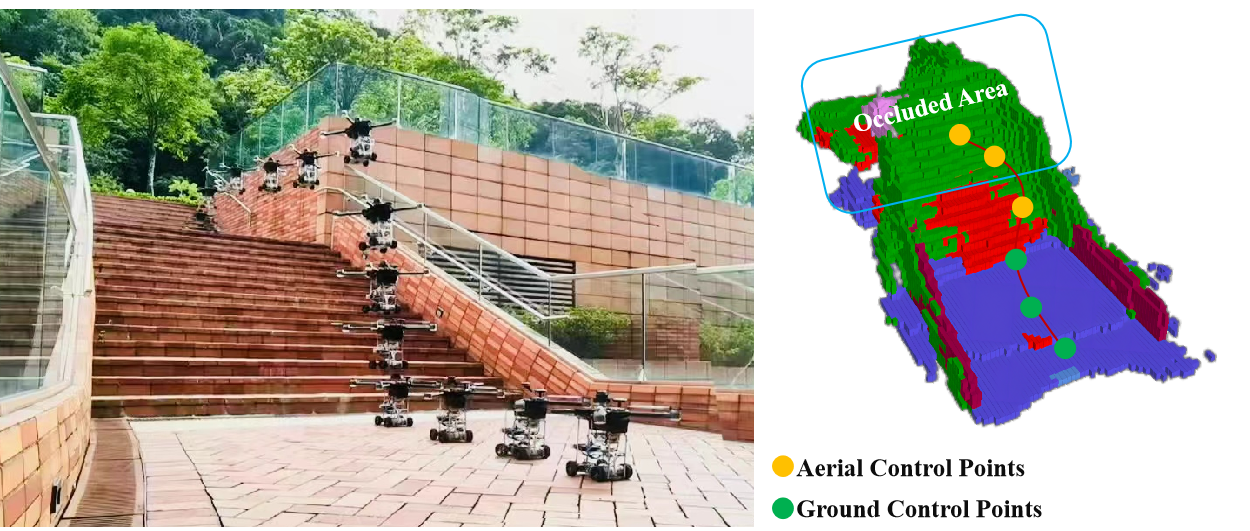
\includegraphics[width=0.8\linewidth]{fig/agrnav.png}}

    % \vspace{-0.2cm}
    \subfloat[Outdoors]{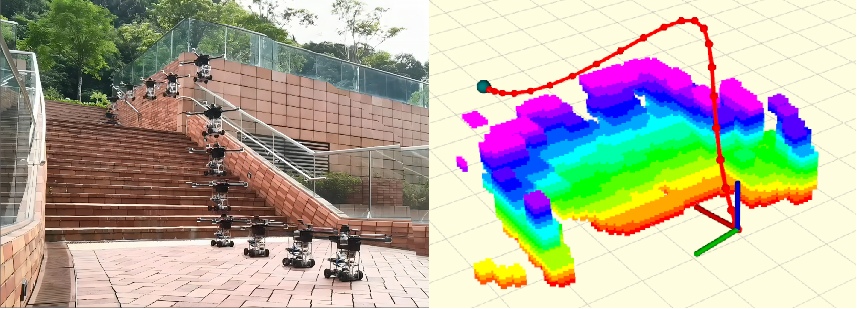
\includegraphics[width=0.8\linewidth]{fig/agr_outdoors.png}}
    
    % \vspace{-0.3cm}
    \caption{By predicting occlusions in advance, AGRNav~\cite{agrnav} gains an accurate perception of the environment and avoids collisions, resulting in efficient and energy-saving paths.}
    \label{fig:agrnav}
    % \vspace{-0.3cm}
\end{figure}


\subsection{End-to-End Performance on Real-World Applications}

\begin{table*}[htb]
    
    \vspace{-0.3cm}
    \renewcommand\arraystretch{0.9}
    \centering
\begin{tabular}{ccc|c|c|c|c|c|c}
\toprule
Model(number & Local compu- & \multirow[c]{2}{*}{System} & \multicolumn{2}{|c|}{Transmission time/s} & \multicolumn{2}{|c|}{Inference time/s} & \multicolumn{2}{c}{Percentage(\%)} \\
of parameters)& tation time/s &  & indoors & outdoors & indoors & outdoors & indoors & outdoors \\
\midrule
\multirow[c]{4}{*}{Kapao(77M)} & \multirow[c]{4}{*}{1.01($\pm$0.03)} & DS & 0.21($\pm$0.1) & 0.24($\pm$0.12) & 0.36($\pm$0.2) & 0.40($\pm$0.17) & 58.33 & 60.21 \\
 &  & DS-C & 0.22($\pm$0.14) & 0.25($\pm$0.12) & 0.32($\pm$0.25) & 0.34($\pm$0.18) & 68.75 & 73.53 \\
 &  & HP & 0.24($\pm$0.15) & 0.28($\pm$0.13) & 0.31($\pm$0.14) & 0.34($\pm$0.12) & 77.42 & 82.35 \\
 &  & Ours & 0.16($\pm$0.13) & 0.21($\pm$0.18) & 0.20($\pm$0.16) & 0.24($\pm$0.20) & 80.09 & 87.56 \\
\cline{1-9} \cline{2-9}
\multirow[c]{4}{*}{AGRNav(0.84M)} & \multirow[c]{4}{*}{0.60($\pm$0.04)} & DS & 0.10($\pm$0.05) & 0.15($\pm$0.05) & 0.41($\pm$0.11) & 0.47($\pm$0.12) & 24.39 & 31.91\\
 &  & DS-C & 0.13($\pm$0.07) & 0.16($\pm$0.06) & 0.38($\pm$0.10) & 0.43($\pm$0.13) & 34.21 & 37.21\\
 &  & HP & 0.24($\pm$0.08) & 0.26($\pm$0.07) & 0.30($\pm$0.09) & 0.33($\pm$0.07) & 78.65 & 79.47 \\
 &  & Ours & 0.18($\pm$0.08) & 0.20($\pm$0.08) & 0.21($\pm$0.16) & 0.25($\pm$0.18) & 86.71 & 80.01 \\
\cline{1-9} \cline{2-9}
\bottomrule
\end{tabular}

    \caption{Average transmission time, inference time, percentage that transmission time accounts for of the total inference time of Kapao and AGRNav in different environments with different systems.}
    \label{tab:e2e_time}
    % \vspace{-0.7cm}
\end{table*}

Table~\ref{tab:e2e_time} shows the end-to-end inference latency and the ratio that transmission time takes up the inference latency and compared with the baselines (we include results of local computation (referred to as Local) for comparison), CacheInf reduced inference latency by 35.5\% to 44.4\% indoors and 29.4\% to 40.0\% outdoors for Kapao and 30.0\% to 48.8\% indoors and 24.2\% to 46.8\% outdoors for AGRNav.
Compared with HP, while CacheInf reduced transmission time by 6 to 8 ms, CacheInf further reduced inference latency by 8 to 10 ms, confirming the effectiveness of the acceleration of the used sparse local operators.
CacheInf's highest percentage that transmission time takes up the inference latency across all cases shows that with shrunk transmission data volume with cache enabled and the integration of HP, CacheInf tend to offload computation to the GPU server more often.
This can also be validated by the increased transmission time and shortened inference latency of DSCCS-C compared with DSCCS.

The reduced inference latency of CacheInf leads to reduction of energy consumed per inference by 25.2\% to 34.3\% indoors and 21.2\% to 34.0\% outdoors for Kapao and 27.4\% to 35.7\% indoors and 21.7\% to 39.9\% outdoors for AGRNav, as shown in Table~\ref{tab:e2e_power}, while the runtime power consumption was increased due to higher frequency of inference.

We report the peak GPU memory consumption on the robot under different strategy in Table~\ref{tab:e2e_mem}: CacheInf (includes both the systems of CacheInf and DSCCS-C), No Cache (includes local computation and HP) and Cache All (a naive strategy that caches the output of every layer).
The results show that CacheInf increased peak GPU memory consumption by 64.6\% for Kapao and 58.5\% for AGRNav compared with no cache, which is however 72.2\% and 81.6\% lower than the cases of Cache All, demonstrating the effectiveness of CacheInf's strategy to reduce the number cached operators.


\begin{table}[htb]
    % \vspace{-0.3cm}
    \renewcommand\arraystretch{0.9}
\tabcolsep=0.095cm
\centering
\begin{tabular}{cc|c|c|c|c}
\toprule
& \multirow[c]{3}{*}{\rotatebox[origin=c]{45}{System}} & \multicolumn{2}{|c}{Power} & \multicolumn{2}{|c}{Energy consumption(J)} \\
& &  \multicolumn{2}{|c}{consumption(W)} & \multicolumn{2}{|c}{per inference}\\
&  & indoors & outdoors & indoors & outdoors \\
\midrule
\midrule
\multirow[c]{5}{*}{\rotatebox[origin=c]{90}{Kapao}} & Local & 9.91($\pm$0.49) & 9.91($\pm$0.49) & 9.79($\pm$0.03) & 9.79($\pm$0.03) \\
 & DS & 6.38($\pm$2.21) & 6.63($\pm$2.38) & 2.30($\pm$0.55) & 2.65($\pm$0.55) \\
 & DS-C & 6.30($\pm$2.15) & 6.53($\pm$2.12) & 2.02($\pm$0.50) & 2.22($\pm$0.53) \\
 & HP & 7.05($\pm$1.63) & 6.94($\pm$0.98) & 2.19($\pm$0.62) & 2.35($\pm$0.42) \\
 & Ours & 7.53($\pm$1.62) & 7.30($\pm$0.96) & 1.51($\pm$0.60) & 1.75($\pm$0.41) \\
\cline{1-6}
\multirow[c]{5}{*}{\rotatebox[origin=c]{90}{AGRNav}} & Local & 8.11($\pm$0.25) & 8.11($\pm$0.25) & 4.86($\pm$0.01) & 4.86($\pm$0.01) \\
 & DS & 6.21($\pm$1.50) & 7.29($\pm$1.55) & 2.55($\pm$0.19) & 3.43($\pm$0.18) \\
 & DS-C & 6.17($\pm$1.56) & 7.00($\pm$1.43) & 2.34($\pm$0.20) & 3.01($\pm$0.20) \\
 & HP & 7.52($\pm$0.51) & 8.04($\pm$0.45) & 2.26($\pm$0.15) & 2.63($\pm$0.15) \\
 & Ours & 7.83($\pm$0.57) & 8.23($\pm$0.56) & 1.64($\pm$0.17) & 2.06($\pm$0.16) \\
\cline{1-6}
\bottomrule
\end{tabular}

    \caption{The power consumption against time (Watt) and energy consumption per inference (Joule) of Kapao and AGRNav different environments with different systems.}
    \label{tab:e2e_power}
    % \vspace{-0.3cm}
\end{table}

\begin{table}[htb]
    
    \renewcommand\arraystretch{0.9}
\centering
\begin{tabular}{c|c|c|c}
\toprule
Model(number & \multicolumn{3}{|c}{Memory Consumption(MB)} \\
 of parameters) & No Cache & Cache All & CacheInf \\
\midrule
Kapao(77M) & 300.6 & 1782.5 & 494.7\\
\hline
AGRNav(0.84M) & 82.8 & 713.3 & 131.2\\
\bottomrule
\end{tabular}

    \caption{Peak GPU memory consumption of different caching strategy on Kapao and AGRNav. }
    \label{tab:e2e_mem}
    \vspace{-0.3cm}
\end{table}

\subsection{Performance on Various Common Models}
The above conclusions can be further validated by results of a wider range of visual models in Table~\ref{tab:torchvision_time} and Table~\ref{tab:torchvision_power}.
Across different visual models, CacheInf reduced the inference latency by 13.4\% to 43.6\% indoors and 13.1\% to 45.9\% outdoors, and it results in the reduction in energy consumed per inference to be 11.1\% to 46.7\% indoors and 9.5\% to 42.2\%
compared with the baselines.
Note that although CacheInf's gain is still evident, the lower bound of CacheInf's gain decreased on these models compared with Kapao and AGRNav; the reason could be that these models are less computation-intensive, which can be implied from their shorter time for local computation compared with Kapao and AGRNav.
When inference of a visual models is not computation-intensive, the gain of using sparse local operators in CacheInf will be limited since execution of each local operator will no longer be the bottleneck.
In terms of GPU memory consumption, CacheInf increased GPU memory consumption by 3.2\% to 24.8\% compared with No Cache, while reducing 12.8\% to 39.5\% GPU memory consumption compared with Cache All.

\begin{table*}[htb]

    \renewcommand\arraystretch{0.9}
    \centering
\begin{tabular}{ccc|c|c|c|c|c|c}
\toprule
 Model(number&  Local compu- & \multirow[c]{2}{*}{System} & \multicolumn{2}{|c|}{Transmission time/ms} & \multicolumn{2}{|c|}{Inference time/ms} & \multicolumn{2}{c}{Percentage(\%)} \\
 of parameters) & taion time/ms &  & indoors & outdoors & indoors & outdoors & indoors & outdoors \\
\midrule
% \multirow[c]{4}{*}{DenseNet(7M)} & \multirow[c]{4}{*}{74.5($\pm$18.7)} & DSCCS & 16.2($\pm$40.9) & 20.8($\pm$51.9) & 81.4($\pm$27.2) & 86.6($\pm$27.7) & 19.95 & 24.07 \\
%  &  & DSCCS-C & 20.4($\pm$43.5) & 25.8($\pm$56.9) & 85.5($\pm$27.9) & 89.6($\pm$29.3) & 23.86 & 28.80 \\
%  &  & HP & 53.4($\pm$34.5) & 52.9($\pm$23.9) & 74.5($\pm$85.7) & 55.1($\pm$15.6) & 71.70 & 96.05 \\
%  &  & CacheInf & 56.3($\pm$37.5) & 57.5($\pm$43.5) & 76.3($\pm$90.6) & 78.1($\pm$33.6) & 73.79 & 73.62 \\
% \cline{1-9} \cline{2-9}
\multirow[c]{4}{*}{RegNet(54M)} & \multirow[c]{4}{*}{175.0($\pm$23.6)} & DSCCS & 47.6($\pm$47.8) & 60.5($\pm$54.0) & 77.8($\pm$39.3) & 86.2($\pm$37.9) & 61.22 & 70.22 \\
 &  & DSCCS-C & 50.7($\pm$49.8) & 62.5($\pm$53.6) & 70.8($\pm$33.3) & 79.5($\pm$39.2) & 71.61 & 78.61 \\
 &  & HP & 49.6($\pm$21.7) & 59.9($\pm$23.4) & 55.0($\pm$24.8) & 64.2($\pm$25.2) & 90.18 & 93.34 \\
 &  & CacheInf & 44.2($\pm$27.7) & 48.5($\pm$25.3) & 45.3($\pm$35.0) & 49.2($\pm$37.2) & 97.57 & 98.58 \\
\cline{1-9} \cline{2-9}
% \multirow[c]{4}{*}{ConvNeXt(88M)} & \multirow[c]{4}{*}{160.2($\pm$21.0)} & DSCCS & 46.9($\pm$43.1) & 56.7($\pm$52.1) & 72.4($\pm$35.7) & 84.7($\pm$36.3) & 64.78 & 66.95 \\
%  &  & DSCCS-C & 48.0($\pm$45.0) & 53.2($\pm$50.1) & 56.8($\pm$28.1) & 70.8($\pm$39.0) & 84.51 & 75.14 \\
%  &  & HP & 50.4($\pm$32.2) & 61.9($\pm$34.8) & 53.9($\pm$26.2) & 65.7($\pm$27.7) & 93.51 & 94.23 \\
%  &  & CacheInf & 40.7($\pm$40.0) & 50.7($\pm$40.3) & 46.7($\pm$35.4) & 56.8($\pm$45.0) & 87.15 & 89.26 \\
% \cline{1-9} \cline{2-9}
\multirow[c]{4}{*}{VGG19(143M)} & \multirow[c]{4}{*}{118.0($\pm$18.9)} & DSCCS & 38.9($\pm$47.1) & 41.6($\pm$53.8) & 65.2($\pm$28.1) & 75.5($\pm$27.1) & 59.75 & 55.09 \\
 &  & DSCCS-C & 42.7($\pm$30.2) & 52.0($\pm$50.3) & 53.2($\pm$33.0) & 60.3($\pm$30.9) & 80.26 & 86.24 \\
 &  & HP & 44.8($\pm$20.9) & 51.5($\pm$15.0) & 47.6($\pm$18.1) & 53.6($\pm$14.7) & 94.15 & 96.07 \\
 &  & CacheInf & 37.8($\pm$31.2) & 43.5($\pm$13.2) & 41.1($\pm$20.3) & 46.6($\pm$12.8) & 94.26 & 93.34 \\
\cline{1-9} \cline{2-9}
\multirow[c]{4}{*}{ConvNeXt(197M)} & \multirow[c]{4}{*}{316.7($\pm$31.0)} & DSCCS & 56.0($\pm$36.1) & 67.0($\pm$37.6) & 79.2($\pm$35.9) & 90.6($\pm$35.4) & 70.72 & 73.98 \\
 &  & DSCCS-C & 56.0($\pm$39.0) & 63.0($\pm$30.2) & 64.7($\pm$40.2) & 68.6($\pm$35.0) & 86.55 & 91.84 \\
 &  & HP & 56.4($\pm$34.7) & 66.5($\pm$33.7) & 59.7($\pm$26.6) & 68.0($\pm$26.6) & 94.43 & 97.88 \\
 &  & CacheInf & 40.4($\pm$37.8) & 46.9($\pm$40.0) & 44.7($\pm$33.3) & 49.0($\pm$30.8) & 90.38 & 95.71 \\
\cline{1-9} \cline{2-9}
\bottomrule
\end{tabular}
    \caption{Average transmission time, inference time, percentage that transmission time accounts for of the total inference time of common visual models in different environments with different systems. }
    \label{tab:torchvision_time}
    % \vspace{-0.5cm}
\end{table*}

\begin{table}[htb]

    % \vspace{-0.3cm}
    \renewcommand\arraystretch{0.9}
\centering
\tabcolsep=0.12cm
\begin{tabular}{cc|c|c|c|c}
\toprule
 & \multirow[c]{3}{*}{\rotatebox[origin=c]{45}{System}} & \multicolumn{2}{|c}{Power} & \multicolumn{2}{|c}{Energy consumption(J)} \\
& &  \multicolumn{2}{|c}{consumption(W)} & \multicolumn{2}{|c}{per inference}\\
 &  & indoors & outdoors & indoors & outdoors \\
\midrule
% \multirow[c]{5}{*}{DenseNet(7M)} & Local & 8.2($\pm$0.27) & 8.2($\pm$0.27) & 0.46($\pm$0.04) & 0.46($\pm$0.04) \\
%  & DS & 6.91($\pm$0.45) & 6.86($\pm$0.46) & 0.56($\pm$0.04) & 0.59($\pm$0.04) \\
%  & DS-C & 7.01($\pm$0.43) & 6.96($\pm$0.43) & 0.60($\pm$0.07) & 0.52($\pm$0.06) \\
%  & HP & 5.36($\pm$0.79) & 5.79($\pm$0.24) & 0.4($\pm$0.06) & 0.32($\pm$0.01) \\
%  & Ours & 6.01($\pm$0.92) & 6.31($\pm$0.56) & 0.46($\pm$0.12) & 0.49($\pm$0.01) \\
% \cline{1-6}
\multirow[c]{5}{*}{\rotatebox[origin=c]{90}{RegNet}} & Local & 9.0($\pm$0.3) & 9.0($\pm$0.3) & 1.37($\pm$0.02) & 1.37($\pm$0.02) \\
& DS & 5.84($\pm$1.79) & 5.36($\pm$1.34) & 0.45($\pm$0.14) & 0.46($\pm$0.12) \\
 & DS-C & 6.04($\pm$1.88) & 5.96($\pm$1.45) & 0.43($\pm$0.16) & 0.47($\pm$0.19) \\
 & HP & 5.24($\pm$1.43) & 5.28($\pm$1.52) & 0.29($\pm$0.08) & 0.34($\pm$0.1) \\
 & Ours & 5.20($\pm$1.51) & 5.23($\pm$1.77) & 0.24($\pm$0.08) & 0.26($\pm$0.09) \\
\cline{1-6}
% \multirow[c]{5}{*}{ConvNeXt(88M)} & Local & 9.7($\pm$0.34) & 9.7($\pm$0.34) & 1.34($\pm$0.02) & 1.34($\pm$0.02) \\
% & DS & 6.01($\pm$0.27) & 5.71($\pm$1.56) & 0.43($\pm$0.05) & 0.48($\pm$0.13) \\
% & DS-C & 6.20($\pm$0.33) & 5.91($\pm$0.21) & 0.35($\pm$0.17) & 0.42($\pm$0.25) \\
%  & HP & 6.68($\pm$1.23) & 6.68($\pm$1.21) & 0.36($\pm$0.07) & 0.44($\pm$0.08) \\
%  & Ours & 6.70($\pm$0.55) & 6.63($\pm$0.26) & 0.31($\pm$0.07) & 0.38($\pm$0.08) \\
% \cline{1-6}
\multirow[c]{5}{*}{\rotatebox[origin=c]{90}{VGG19}} & Local & 9.78($\pm$0.34) & 9.78($\pm$0.34) & 0.95($\pm$0.02) & 0.95($\pm$0.02) \\
& DS & 6.58($\pm$2.14) & 6.93($\pm$2.35) & 0.43($\pm$0.14) & 0.52($\pm$0.18) \\
 & DS-C & 6.82($\pm$2.10) & 7.23($\pm$2.45) & 0.36($\pm$0.18) & 0.43($\pm$0.30) \\
 & HP & 6.51($\pm$1.74) & 7.32($\pm$1.52) & 0.31($\pm$0.08) & 0.39($\pm$0.08) \\
 & Ours & 6.70($\pm$1.88) & 7.22($\pm$1.36) & 0.27($\pm$0.10) & 0.34($\pm$0.09) \\
\cline{1-6}
\multirow[c]{5}{*}{\rotatebox[origin=c]{90}{ConvNeXt}} & Local & 9.92($\pm$0.38) & 9.92($\pm$0.38) & 3.12($\pm$0.03) & 3.12($\pm$0.03) \\
& DS & 5.06($\pm$0.31) & 5.02($\pm$0.37) & 0.4($\pm$0.02) & 0.45($\pm$0.03) \\
 & DS-C & 4.86($\pm$0.44) & 4.99($\pm$0.39) & 0.31($\pm$0.05) & 0.34($\pm$0.09) \\
 & HP & 4.57($\pm$0.23) & 4.54($\pm$0.25) & 0.27($\pm$0.01) & 0.31($\pm$0.02) \\
 & Ours & 5.26($\pm$0.40) & 5.39($\pm$0.27) & 0.24($\pm$0.05) & 0.26($\pm$0.04) \\
\cline{1-6}
\bottomrule
\end{tabular}
    \caption{The power consumption against time (Watt) and energy consumption per inference (Joule) of common visual models in different environments with different systems.}
    \label{tab:torchvision_power}
    % \vspace{-0.3cm}
\end{table}

\begin{table}[htb]
    
    \vspace{-0.3cm}
    % \renewcommand\arraystretch{0.9}
    \centering
    \begin{tabular}{c|c|c|c}
    \toprule
    Model(number & \multicolumn{3}{|c}{Memory Consumption(MB)} \\
     of parameters) & No Cache & Cache All & CacheInf \\
    \midrule
    % DenseNet(7M) & 30.8 & 159.7 & 53.2\\
    % \hline
    RegNet(54M) & 207.5 & 427.7 & 258.9\\
    \hline
    % ConvNeXt(88M) & 337.9 & 603.9 & 369.9\\
    % \hline
    VGG19(143M) & 548.1 & 668.7 & 582.8\\
    \hline
    ConvNeXt(197M) & 765.4 & 1152.7 & 789.8 \\
    \bottomrule
    \end{tabular}
    
        \caption{Peak GPU memory consumption of different caching strategy on common visual models. }
        \label{tab:torchvision_mem}
    \vspace{-0.3cm}
\end{table}

\subsection{Micro-Event}
We first present the micro-events about the real-time inference latency of Kapao of different systems under fluctuating bandwidth in Figure~\ref{fig:micro_e2e}.
And we can learn that CacheInf consistently achieved the lowest inference latency among all the systems and the gain was most significant under lower bandwidth.
Then we fixed the wireless network bandwidth to 48Mb/s and examined different systems's performance at varied cache ratios from a sequence of video images in Figure~\ref{fig:micro_ratio}: at high cache ratios, CacheInf dramatically reduced inference latency compared with other baselines; at low cache ratios, CacheInf degraded to Hybrid-Parallel or even slightly increased inference latency compared with Hybrid-Parallel, and the reason could be the overhead to analyze reusable cache and update cache.
We can also observe when cache ratios fluctuated, the inference latency of CacheInf was more stable than DSCCS-C, which can be attributed to CacheInf's ability to adjust input ratio ($x$) to reduce inference latency.

\begin{figure}[htb]
    % \vspace{-0.3cm}
    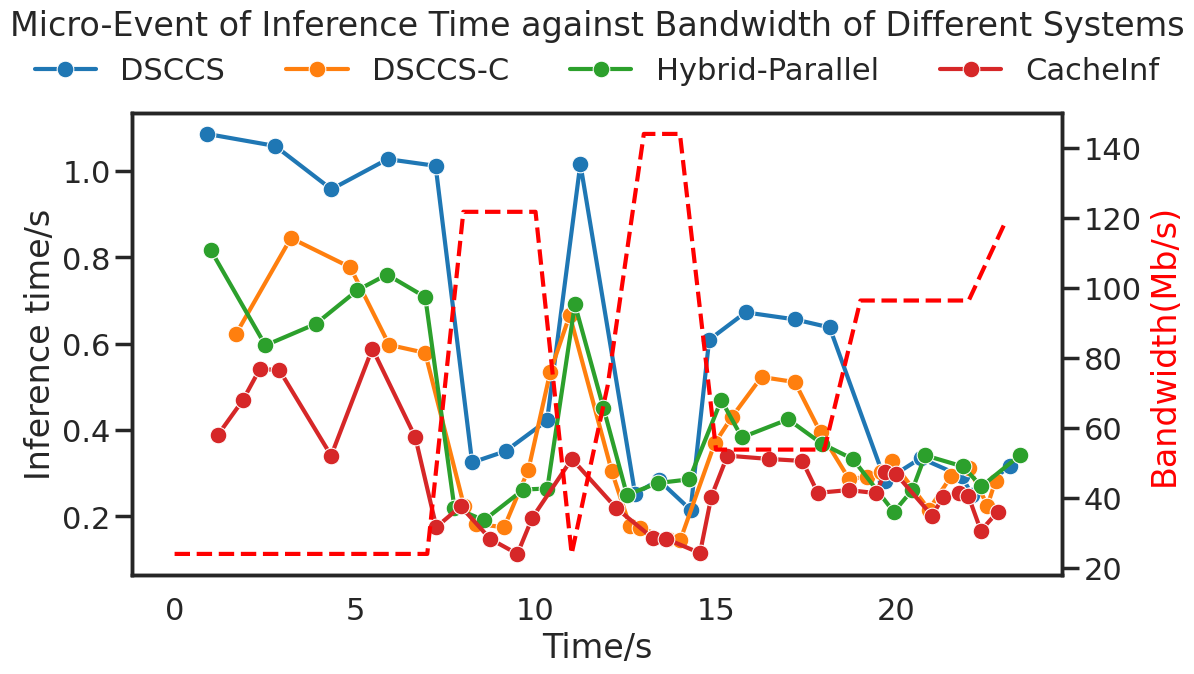
\includegraphics[width=0.8\linewidth]{fig/MicroEvent2.png}
    % \vspace{-0.3cm}
    \caption[short]{Kapao: inference latency of different systems at different wireless network bandwidth.}
    \label{fig:micro_e2e}
    % \vspace{-0.3cm}
\end{figure}


\begin{figure}[htb]
    % \vspace{-0.3cm}
    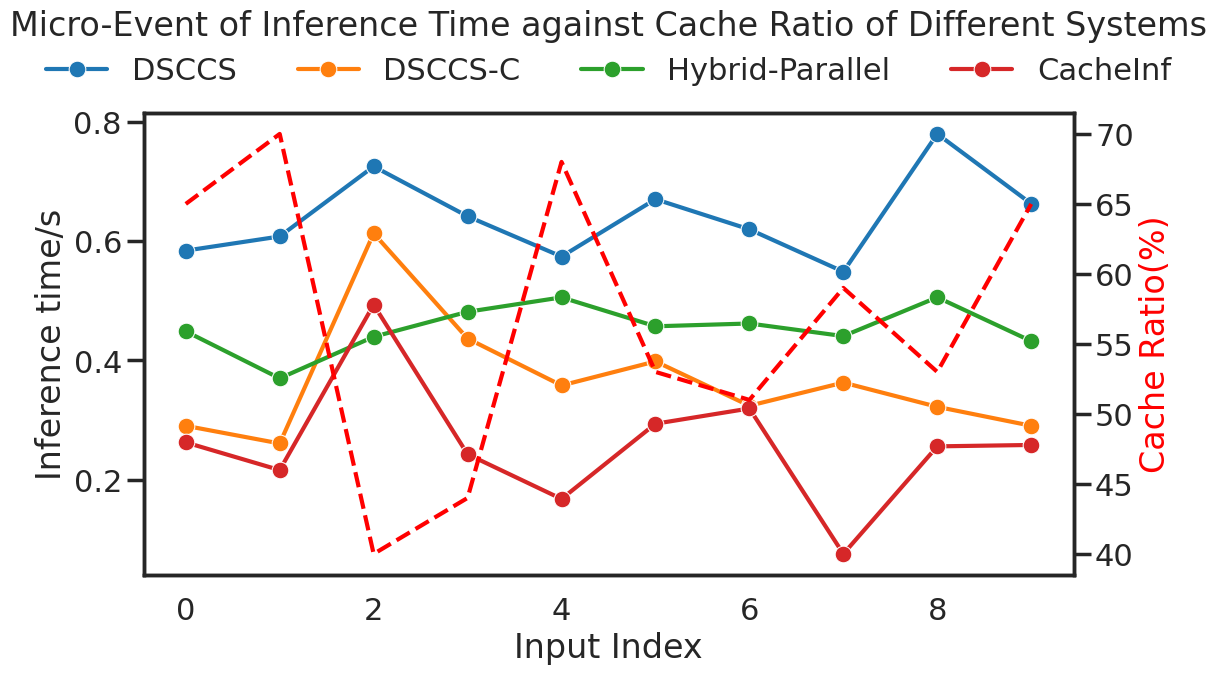
\includegraphics[width=0.8\linewidth]{fig/MicroEvent3.png}
    % \vspace{-0.3cm}
    \caption[short]{Kapao: inference latency of different systems at different cached ratio with fixed wireless network bandwidth.}
    \label{fig:micro_ratio}
    % \vspace{-0.3cm}
\end{figure}

\subsection{Sensitivity}

\begin{table}[htb]
    \begin{tabular}{c|c|c|c|c}
        \toprule
        \multirow[c]{2}{*}{Model} & \multirow[c]{2}{*}{Statistics} & \multicolumn{3}{c}{Difference Filtering Threshold (N)} \\
        \cline{3-5}
        & & 0.1 & 0.2 & 0.3 \\
        \midrule
        \multirow[c]{2}{*}{Kapao} & inference latency & & & \\
            & accuracy (AP) & 75.8 & 74.6 & 72.5 \\
        \hline
        \multirow[c]{2}{*}{AGRNav} & inference latency & & & \\
            & accuracy () & & & \\
        \hline
        \multirow[c]{2}{*}{ConvNeXt} & inference latency & & & \\
            & accuracy () & & & \\
        \bottomrule

    \end{tabular}
    \caption[accuracy]{How different difference filter threshold (N) for identifying reusable cache affects the inference latency of CacheInf and the accuracy of visual models.}
\end{table}

% \subsection{Sampling Rate of Video Frames}

% \begin{table*}[htb]
%     \begin{tabular}{c|c|c|c|c}
%         \toprule
%         \multirow[c]{2}{*}{Model} & \multirow[c]{2}{*}{Statistics} & \multicolumn{3}{|c}{Sampling rate} \\
%         \cline{3-5}
%         & & 1 & 2 & 4 \\
%         \midrule
%         \bottomrule

%     \end{tabular}
%     \caption[sample rates]{How the sampling rate of video frames influence the performance of CacheInf.}
% \end{table*}

\subsection{Discussion}
From the above results we can learn that CacheInf is fundamentally trading-off between GPU memory with inference latency, just as systems in other domains with cache enabled.
Since the resulting increased GPU memory consumption may be unfavorable for devices with tight memory budget, adjusting such trade-off to further reduce extra GPU memory consumption to fit in these devices will be our future work.
Another limitation of CacheInf is that it relies on continuity of input and thus is unsuitable for scenarios where the perspective of the robot changes dramatically.
\label{sec:eva}




\section{Conclusion}
In this paper, we present CacheInf, a collaborative edge-cloud cache system for efficient robotic visual model inference.
Based on the continuity of visual input of robots in the field and the local operators commonly used in visual models, we introduce cache mechanism to visual model inference in CacheInf.
By reusing computation results of similar local geometries between consecutive inputs, CacheInf accelerates visual model inference by reducing both local computation time and transmission time when offloading computation to the GPU server.
The more real-time visual model inference on robots enabled by CacheInf will nurture more visual models to be deployed in real-world robots.




\bibliographystyle{plain}
\bibliography{references}

\end{document}
\endinput
%%
%% End of file `sample-sigplan.tex'.
